%!TEX root = ../main.tex
\section{Real-word data experiment on Yahoo! Front Page}
\label{sec:yahoo}
\paragraph{R6A - Yahoo! Front page today module user click log dataset.} 
This dataset was used for the Exploration and Exploitation Challenge\footnote{\url{http://explochallenge.inria.fr/}} at ICML 2012 and inspired new algorithms. Among them, we mention the work of \citet{traca2015regulating} who noticed the non-stationary trend and took advantage of it. Since then the dataset continues to be a benchmark\footnote{As it allows for offline evaluations as the actions were samples uniformly.} for non-stationary bandits \citep{liu2018change-detection,cao2019nearly}. It contains the history of clicks on news articles of 45 million users in the first ten days of May 2009. We use three features in this dataset: \textit{timestamp} (rounded every 5 minutes), \textit{article$\!\_\!$id}, and \textit{click}. 
 
\paragraph{A real decaying scenario.} Every day, between 6 pm and 6 am EST (12 hours), we notice a decreasing trend in click probability. It suggests that people in the US read less and less news during the evening and night. For each day, we keep all the articles that have been recommended at every timestamp during the 12 hours. For these articles, we use a rolling average window of 30000 in order to estimate the probability of click for each article at each timestamp \footnote{For each timestamp, we average the values given by rolling average. These values are close to each other because the number of click opportunities per article in the same timestamp is small compared to 30000.}. We use the \underline{real} total traffic for each timestamp. We highlight that \textit{we do not enforce any of our assumptions} to create reward functions to be aligned with our setup. In particular, we do not enforce them to be piecewise constant nor to be decreasing. At each round, the learner receives 10 reward samples in order to reduce the cost of computation.

\paragraph{Algorithms and Parameters.} We include two versions of \FEWA and \RAWUCB: with the theoretical tuning $\alpha =4$; and with the empirical tuning $\alpha_{\mathrm{R}} = 1.4$ and $\alpha_{\mathrm{F}} = 0.06$. These two values were selected on the rested benchmark (c.f. Section~\ref{sec:rested-experiment}). This benchmark has 30 different problems (for different $L$) but the best tuning of $\alpha$ is the same for all the considered problems. We replace \RAWUCB and \FEWA with their efficient versions because of the longer horizon. 

We also include \EXPS\citep{auer2002nonstochastic} and \GLRUCB \citep{besson2019generalized}.  For \EXPS, we use the theoretical tuning which requires the knowledge of $T$ and $V_T$. \GLRUCB has two parameters: a confidence level $\delta$ for its change-point detector and an active exploration rate $\alpha$. We set $\alpha$ to zero. Indeed, the active exploration of change-detection algorithms is only useful in the increasing case (as argued by \citet{cao2019nearly}). We tune $\delta$ by its theoretical value, which requires the knowledge of $T$. Last, we only restart the history of the changed arm as our setup does not assume that all the rewards change simultaneously. For a fair comparison, we only use the subgaussian version of the algorithm. Indeed, KL-UCB indexes are expensive to compute. Instead, for all the confidence bound algorithms, we rather tune $\sigma^2 = 1$ in the rested benchmark and $\sigma^2 = 0.29$ in the restless benchmark (the variance of a binomial $\mathcal{B}\pa{10,0.03)}$.  

We do not include \SWA \citep{levine2017rotting} which was shown to be less consistent than \FEWA and \RAWUCB on rested rotting bandits. We do not include \SWUCB and \DUCB as they were shown to be unable to learn in the rested setting  \citep{levine2017rotting, seznec2019rotting}. We also do not include \CUSUMUCB \citep{liu2018change-detection} and \MUCB \citep{cao2019nearly}, as 1) they were shown to under-perform against \GLRUCB \citep{besson2019generalized}; and 2) their change-detector is harder to tune.

Note that our goal is to compare algorithms with the same tuning in the rested and restless benchmark. 

\paragraph{Results.} We display the results for eight different days in Figure~\ref{fig:restless-exp}.%TODO add day 10?
We will comment day~2 and day~7. On day~2, there are several switches of optimal arms with many near-optimal ones: tracking the best arm is a "hard" problem. On day~7, one arm consistently dominates the others by far. Hence, it is an "easy" case where good algorithms should have a logarithmic regret rate. We also display the running time of each algorithm in Table~\ref{tab:restless-time}.

 \begin{figure*}[p!]
\caption{\textbf{Left:} reward functions from the Yahoo! dataset \\ \textbf{Right:} average regret of policies over 500 runs}
\label{fig:restless-exp}
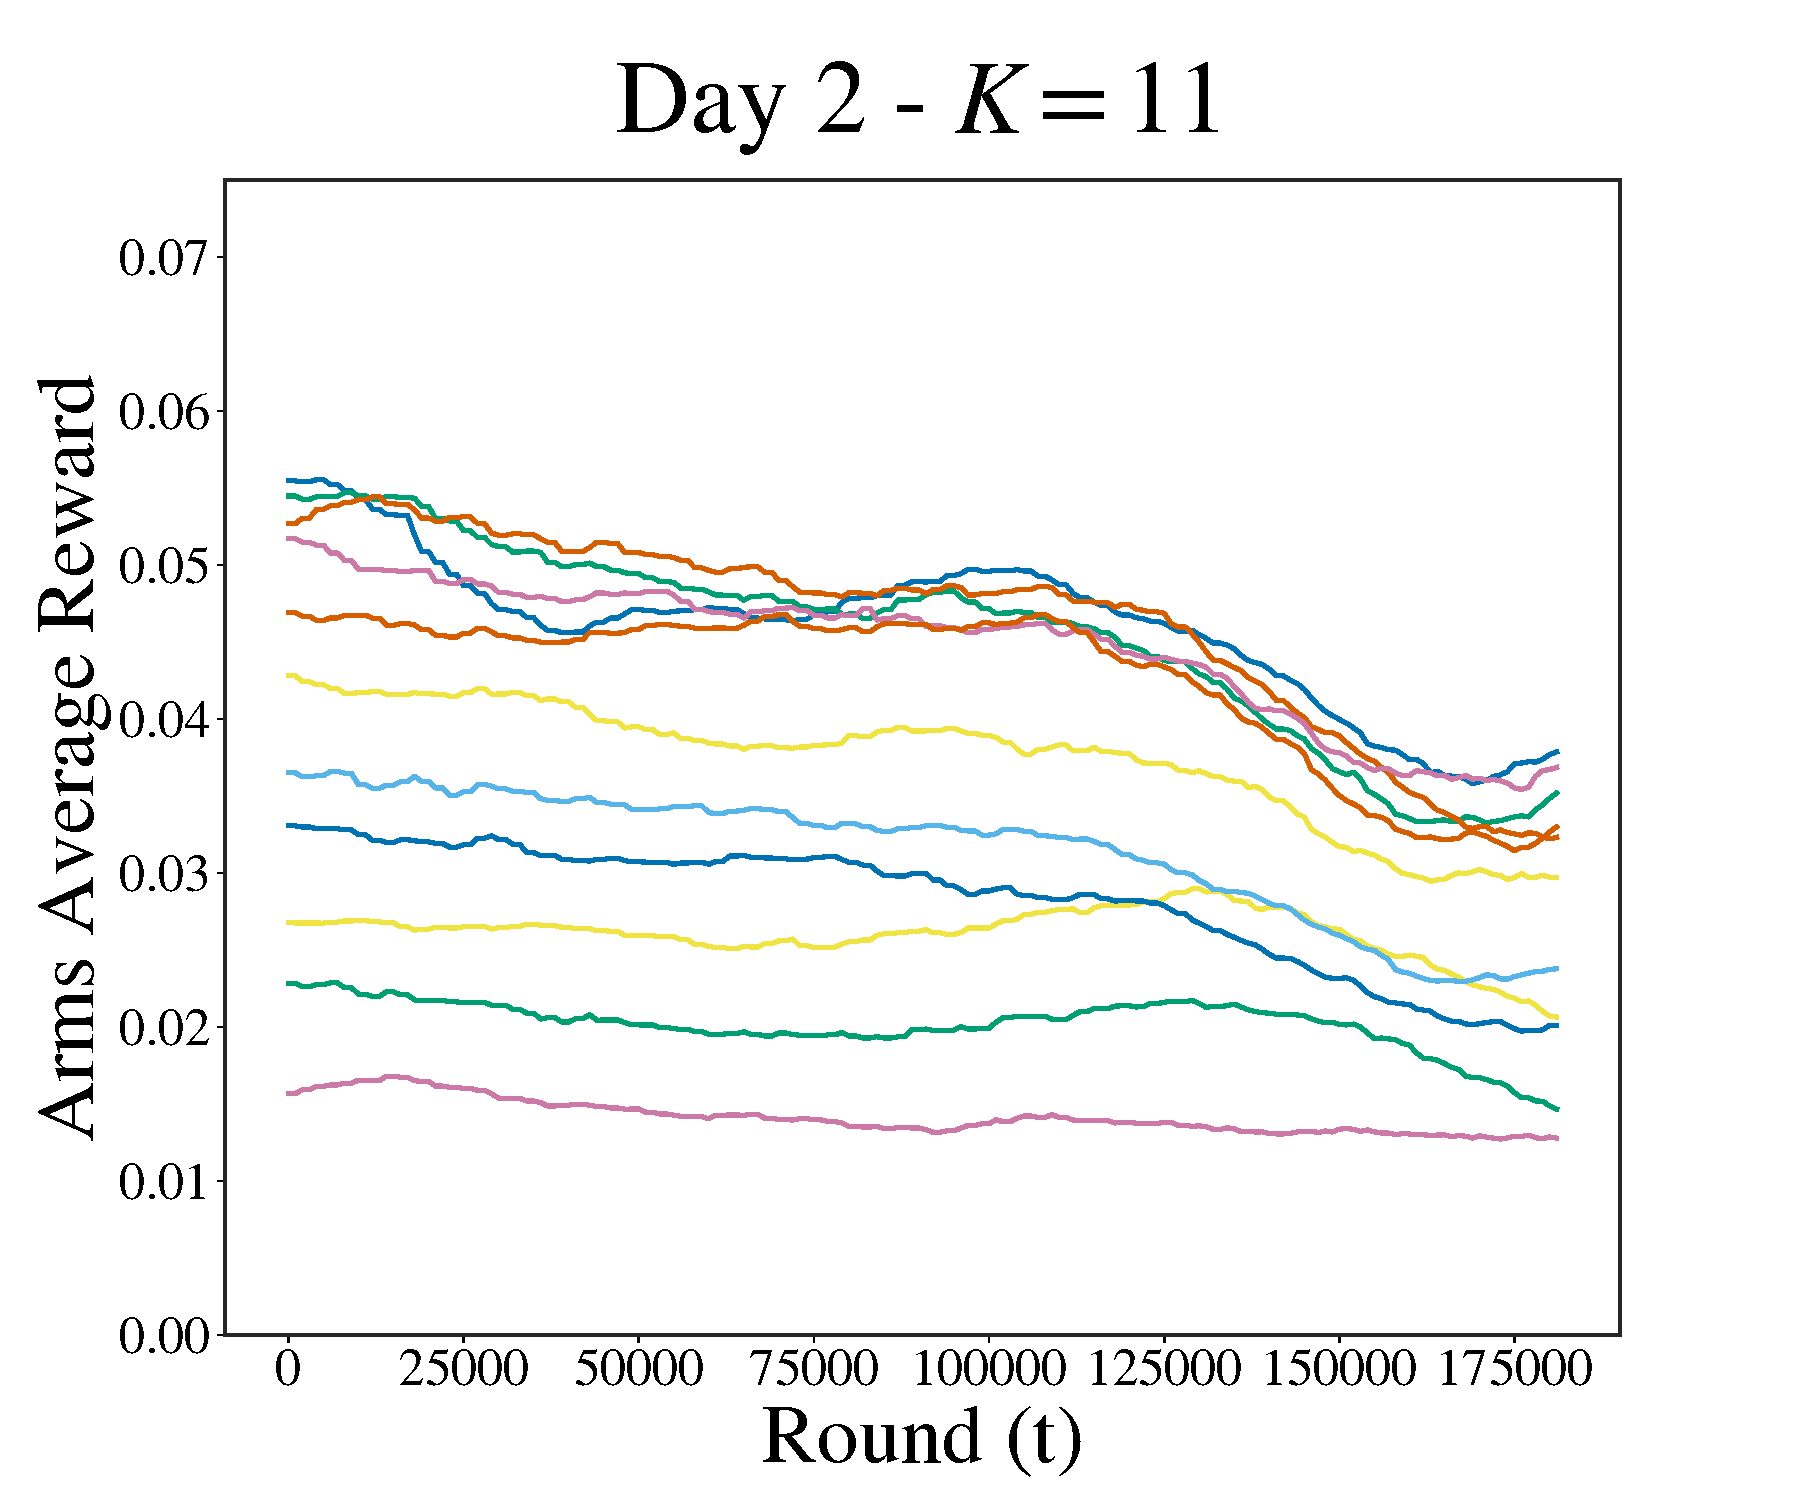
\includegraphics[clip, width= 0.495\textwidth]{4Restless/fig/reward_plot_day2.pdf}
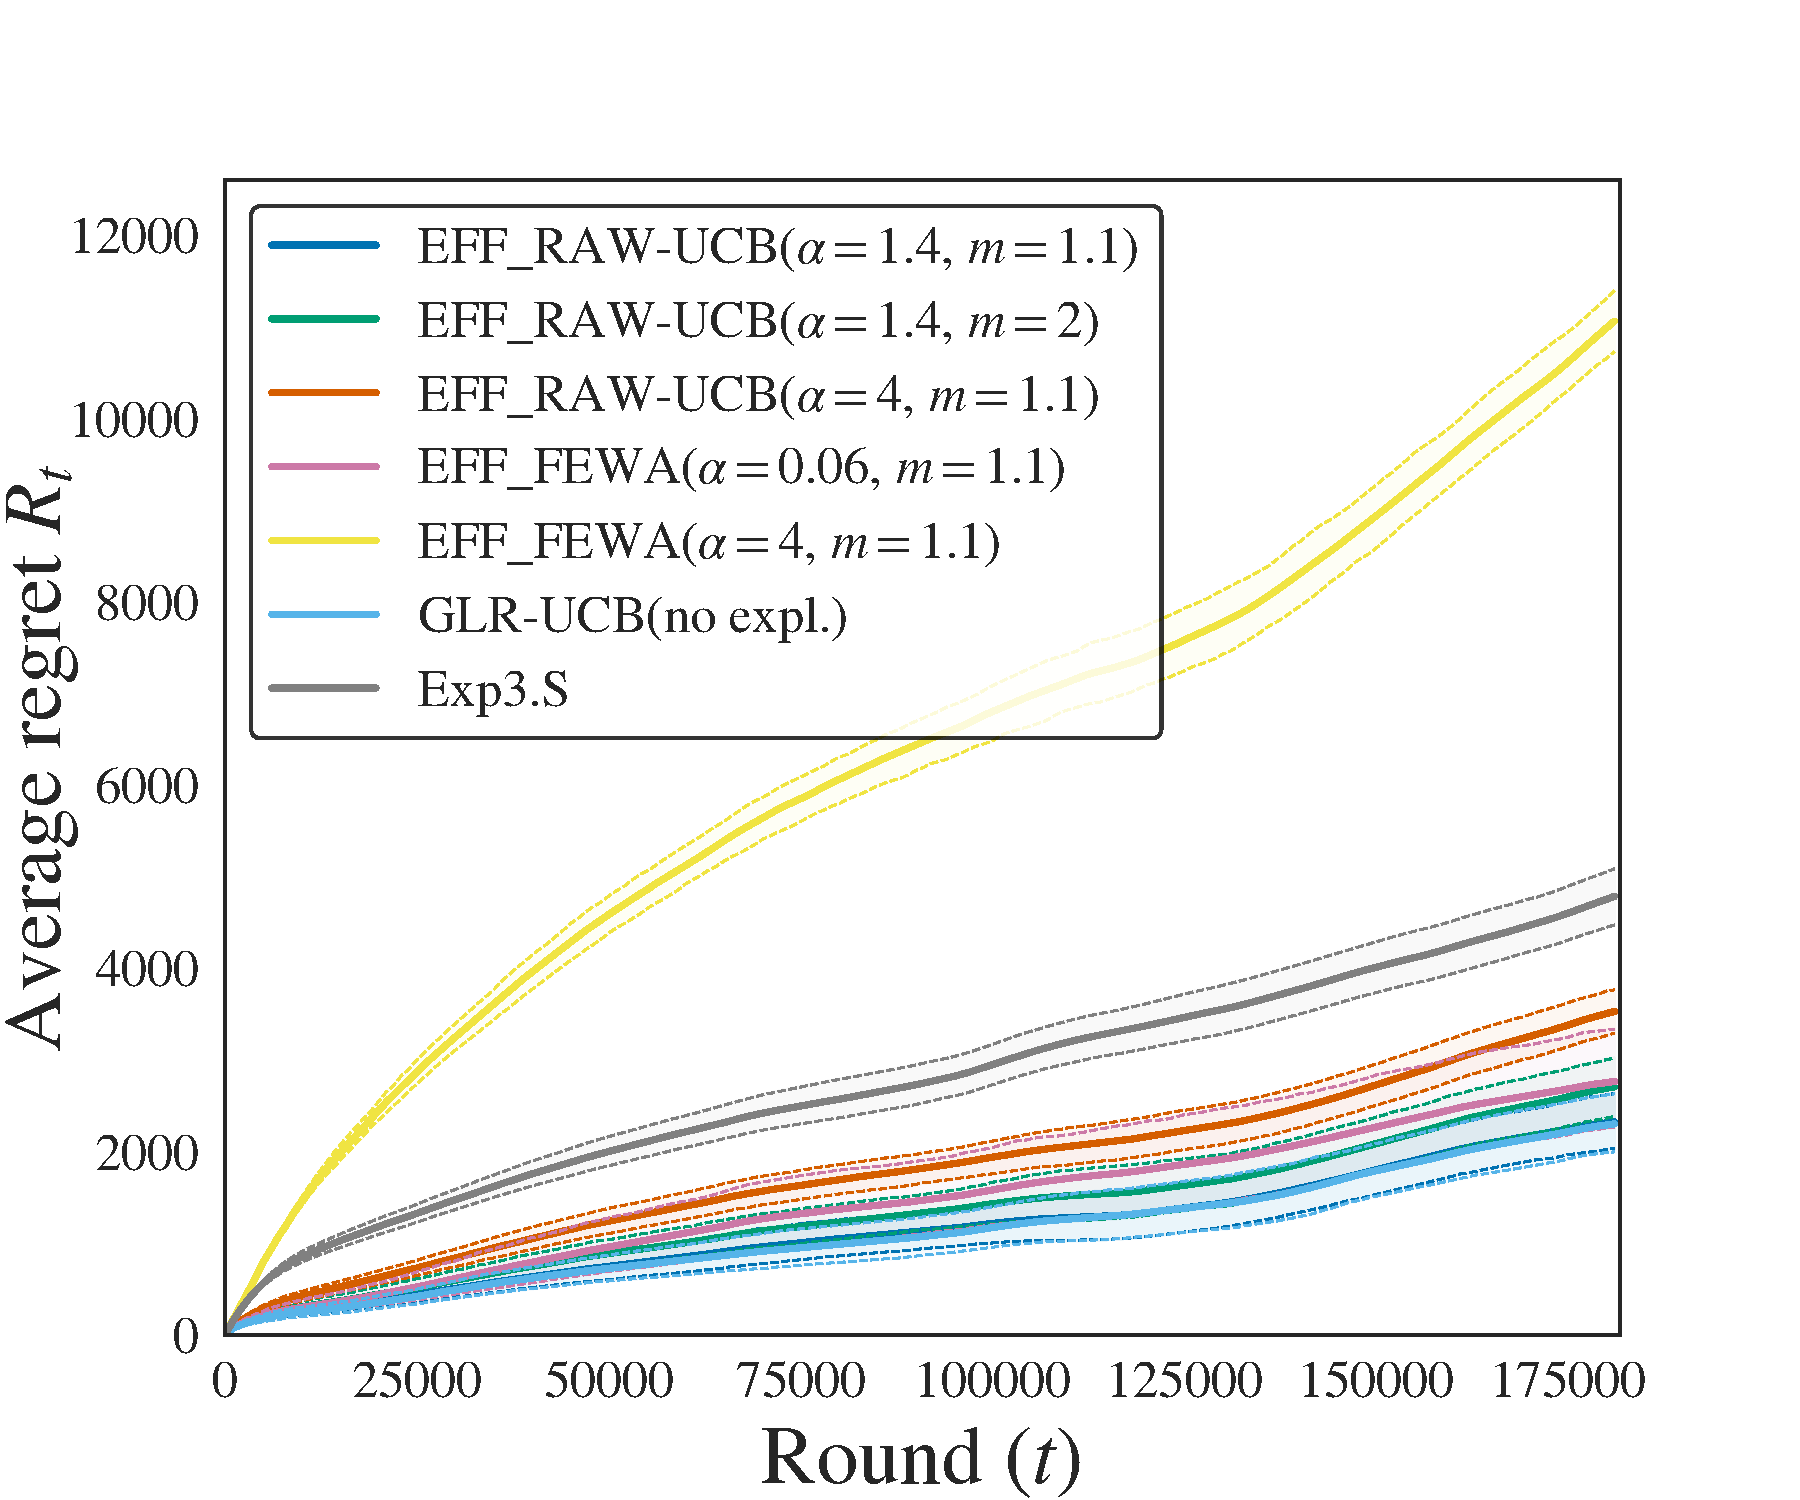
\includegraphics[clip, width= 0.495\textwidth]{4Restless/fig/DAY2.pdf}
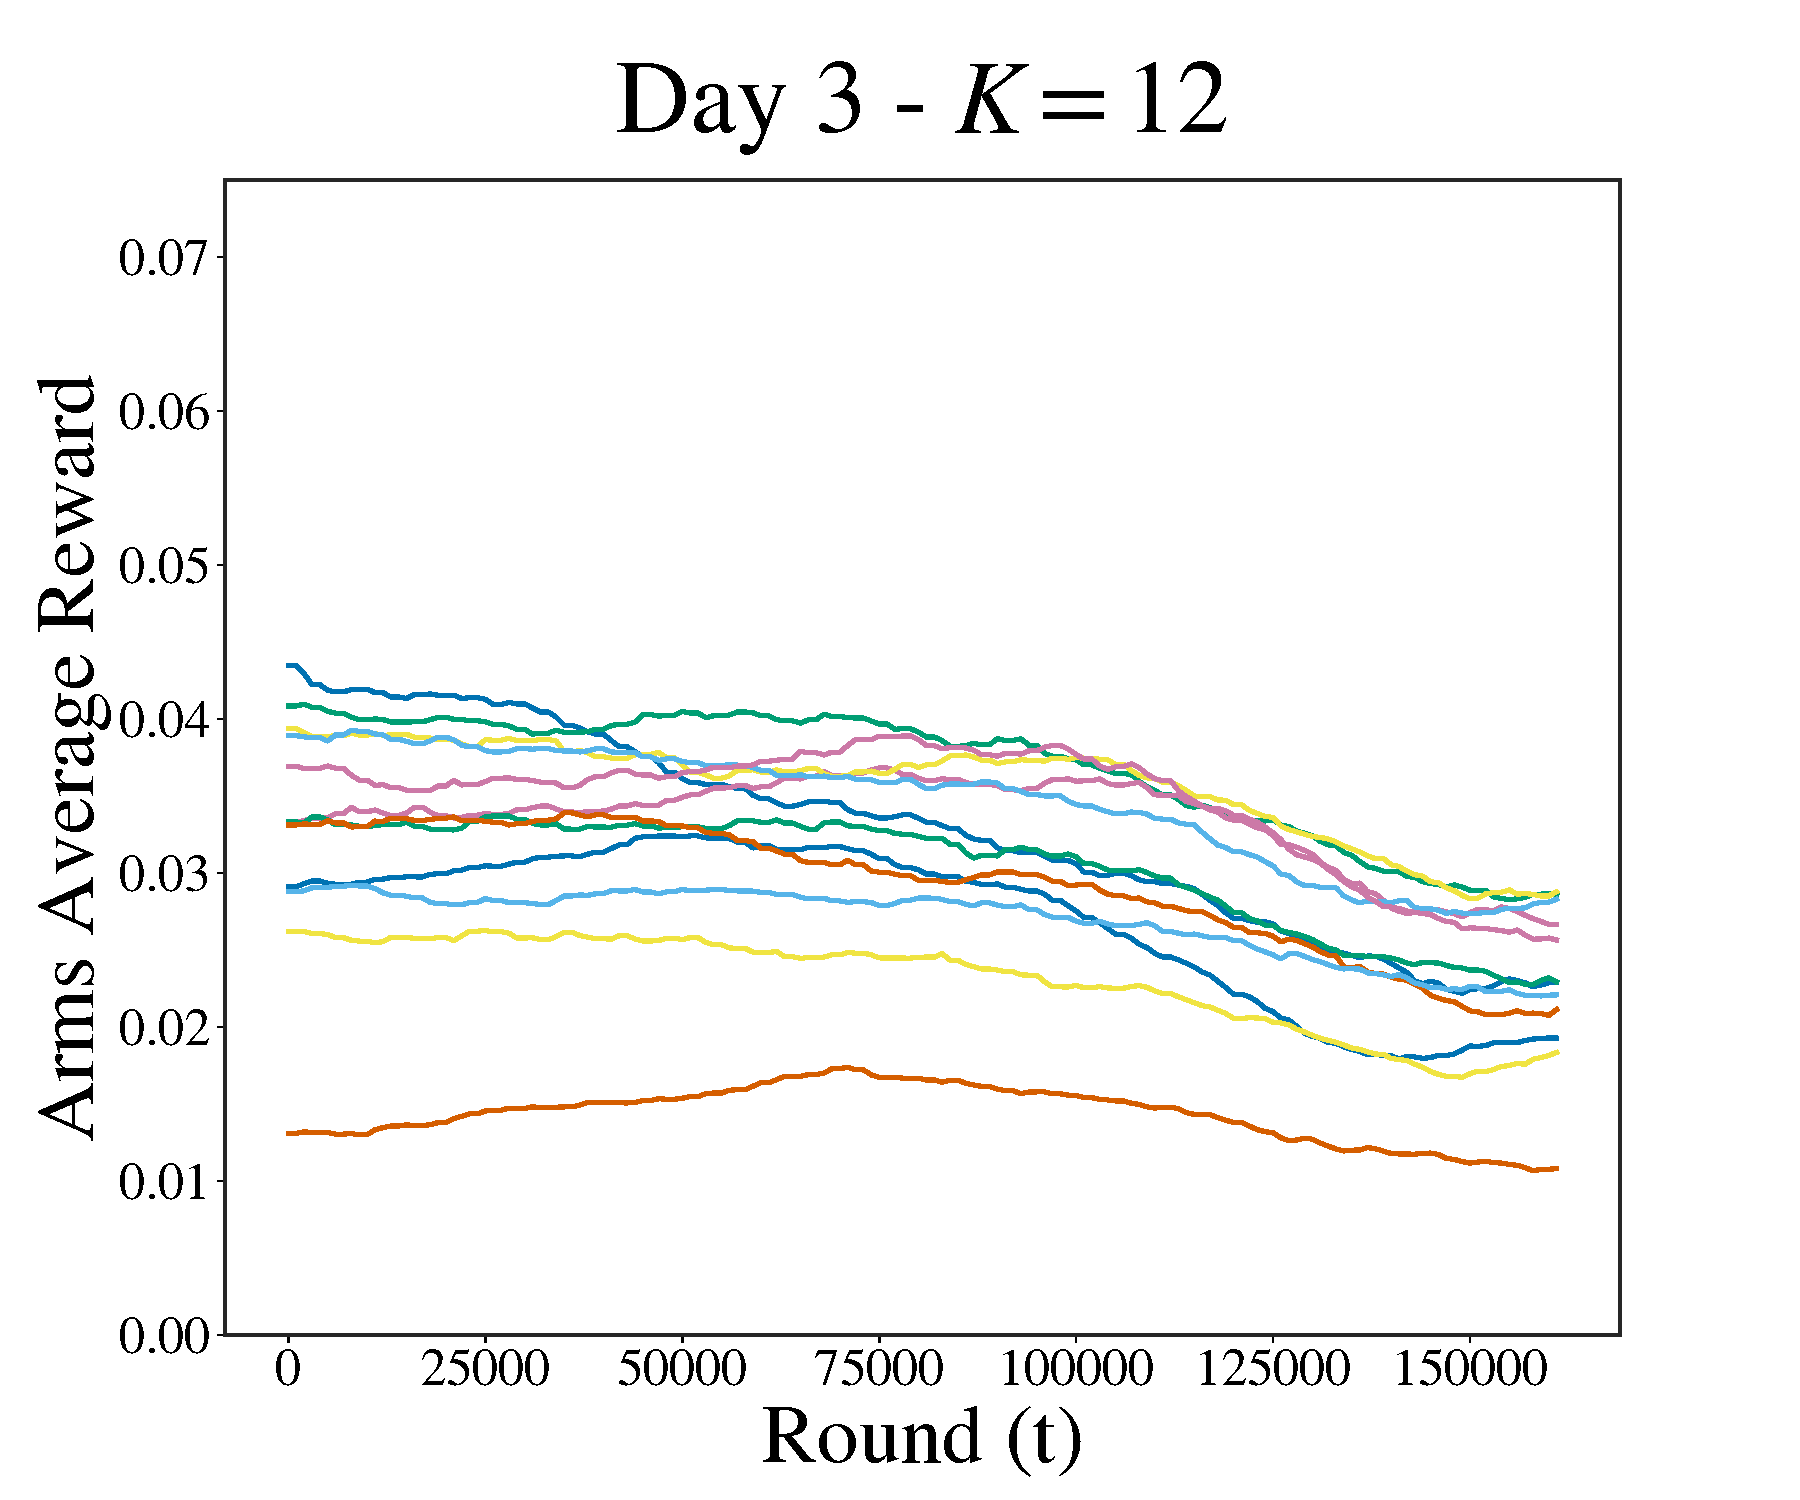
\includegraphics[clip, width= 0.495\textwidth]{4Restless/fig/reward_plot_day3.pdf}
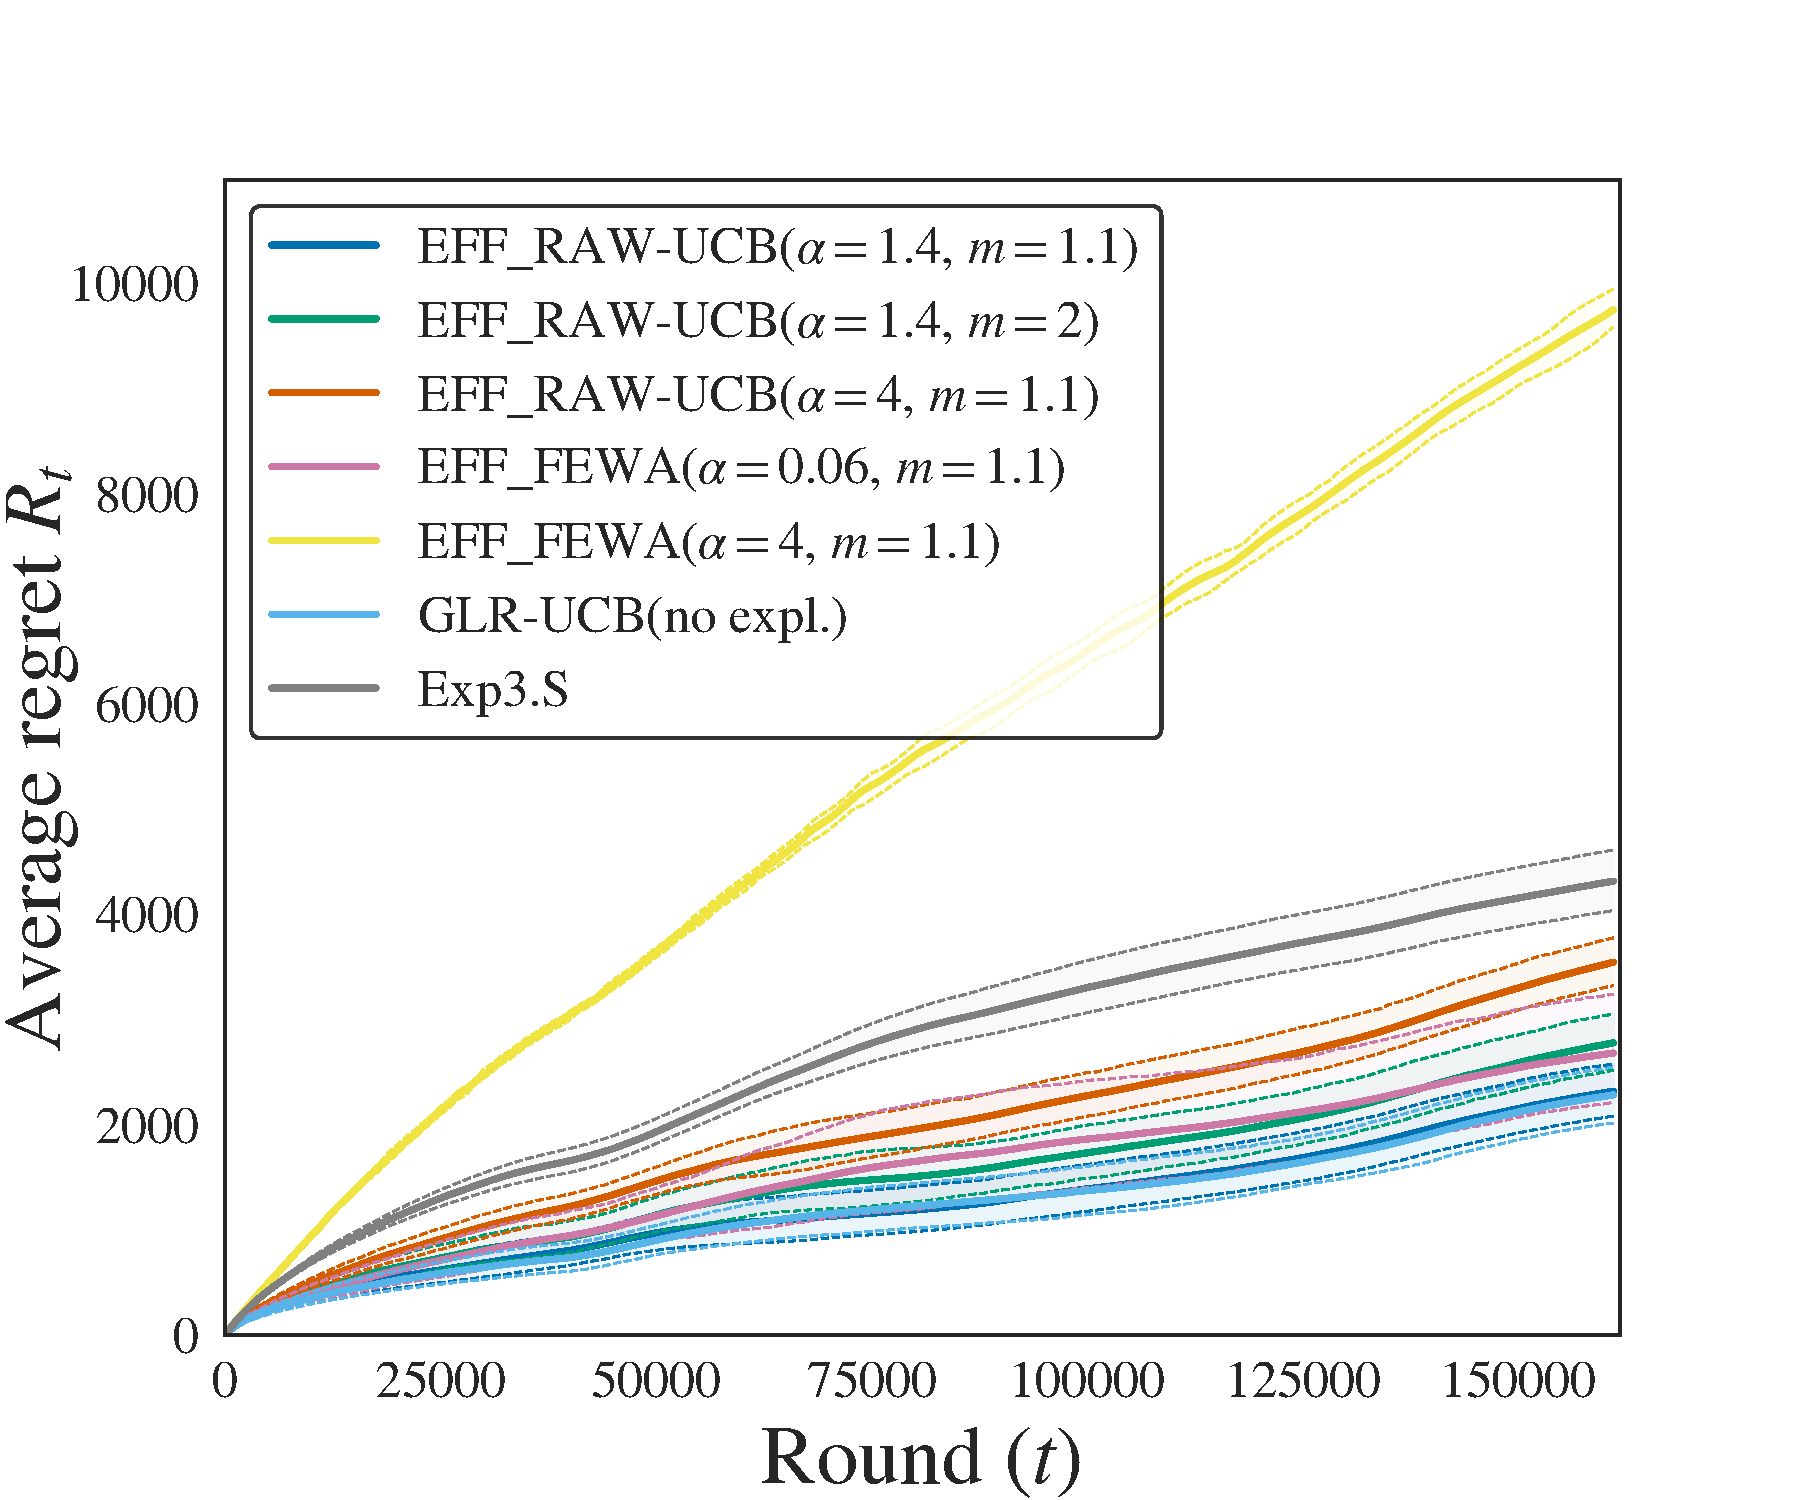
\includegraphics[clip, width= 0.495\textwidth]{4Restless/fig/DAY3.pdf}
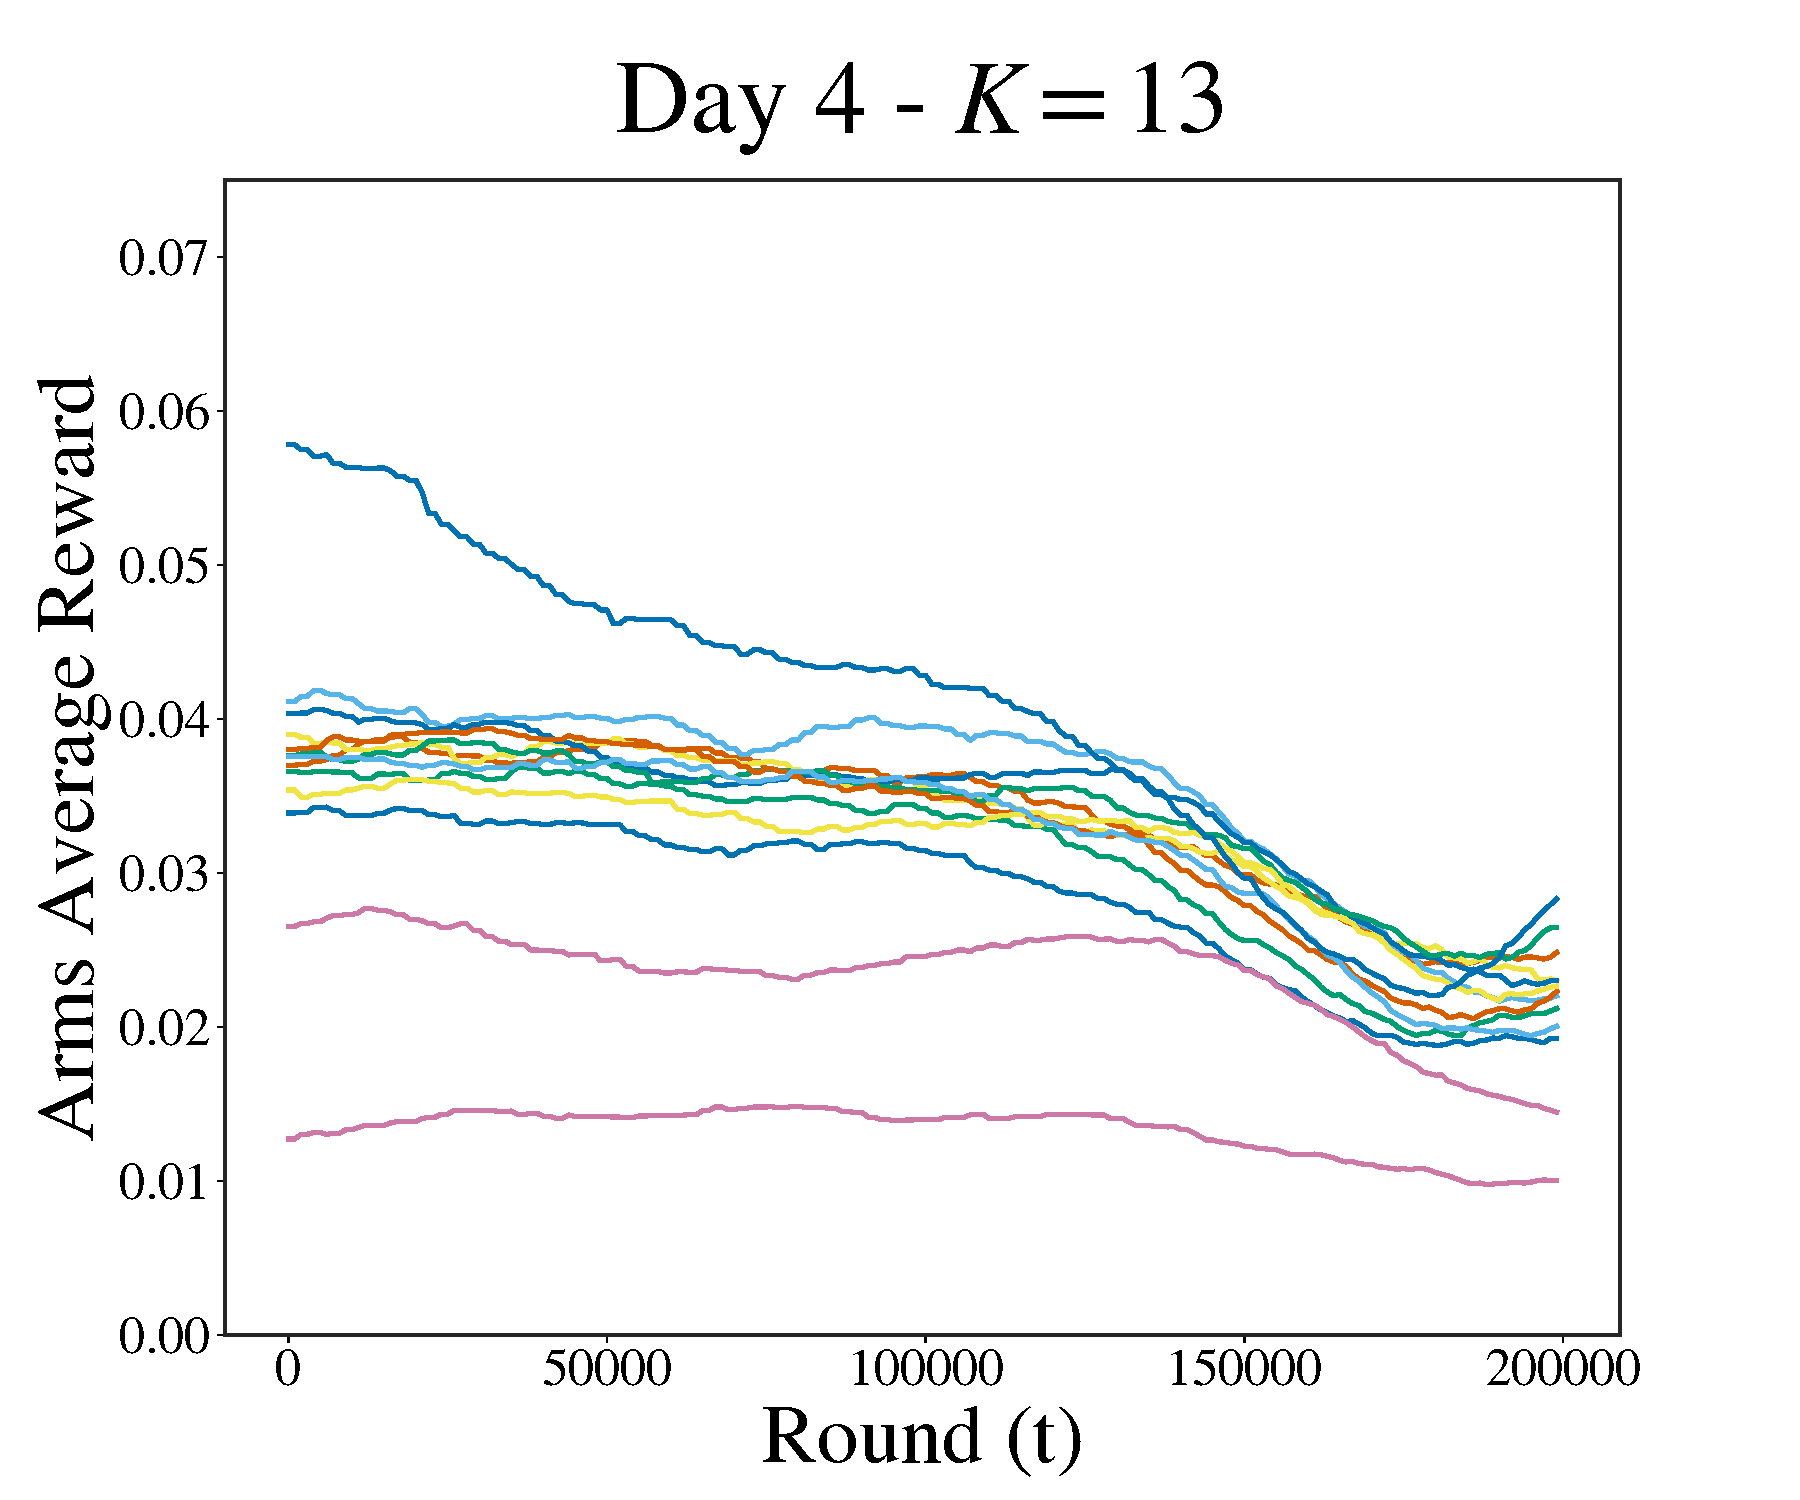
\includegraphics[clip, width= 0.495\textwidth]{4Restless/fig/reward_plot_day4.pdf}
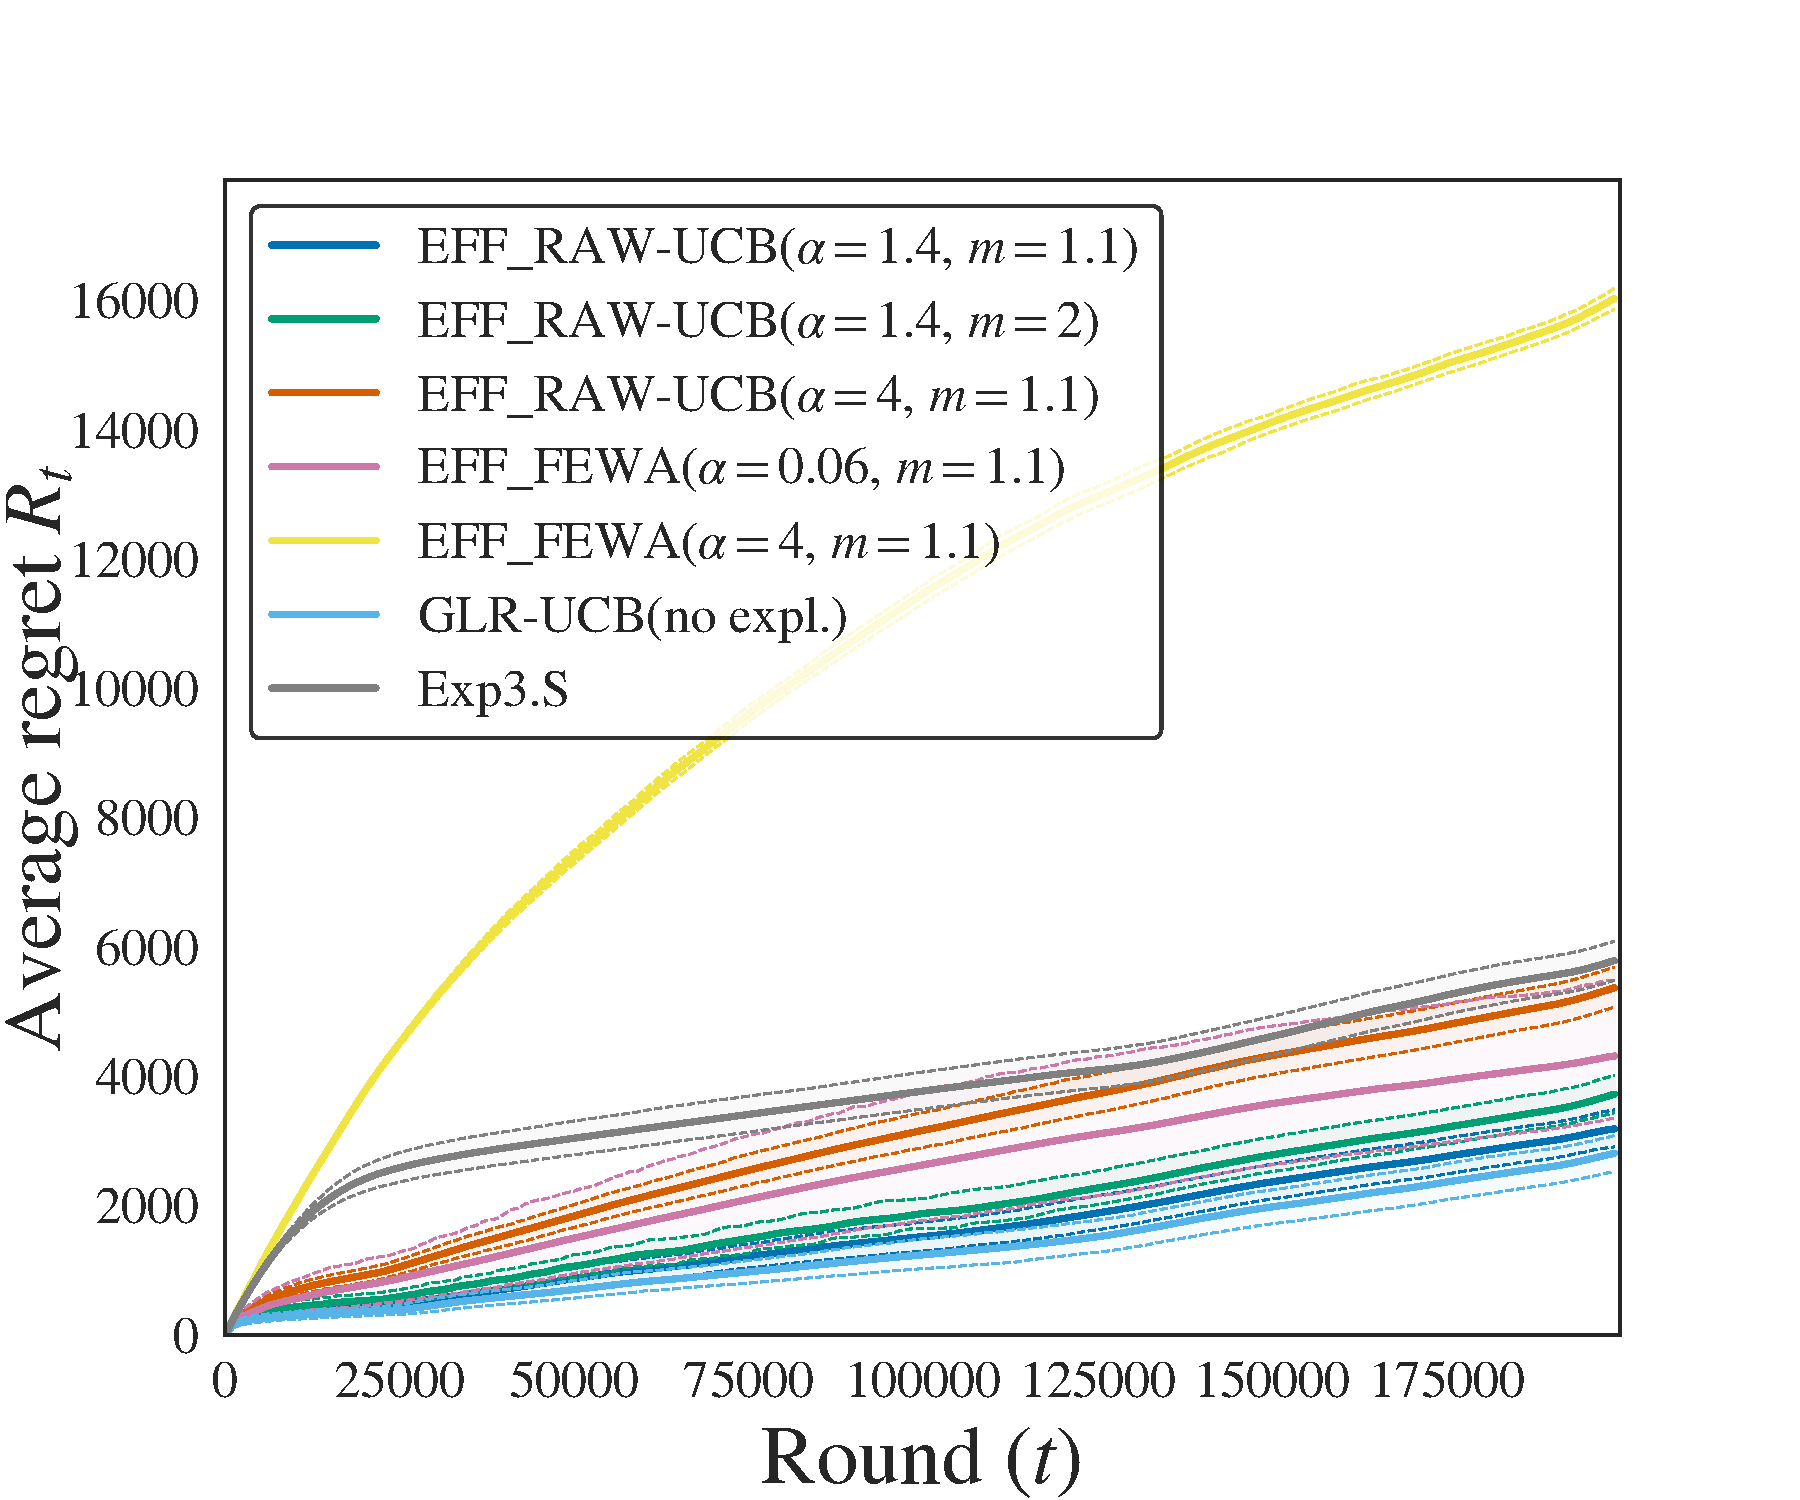
\includegraphics[clip, width= 0.495\textwidth]{4Restless/fig/DAY4.pdf}
\end{figure*}

\begin{figure*}[p!]
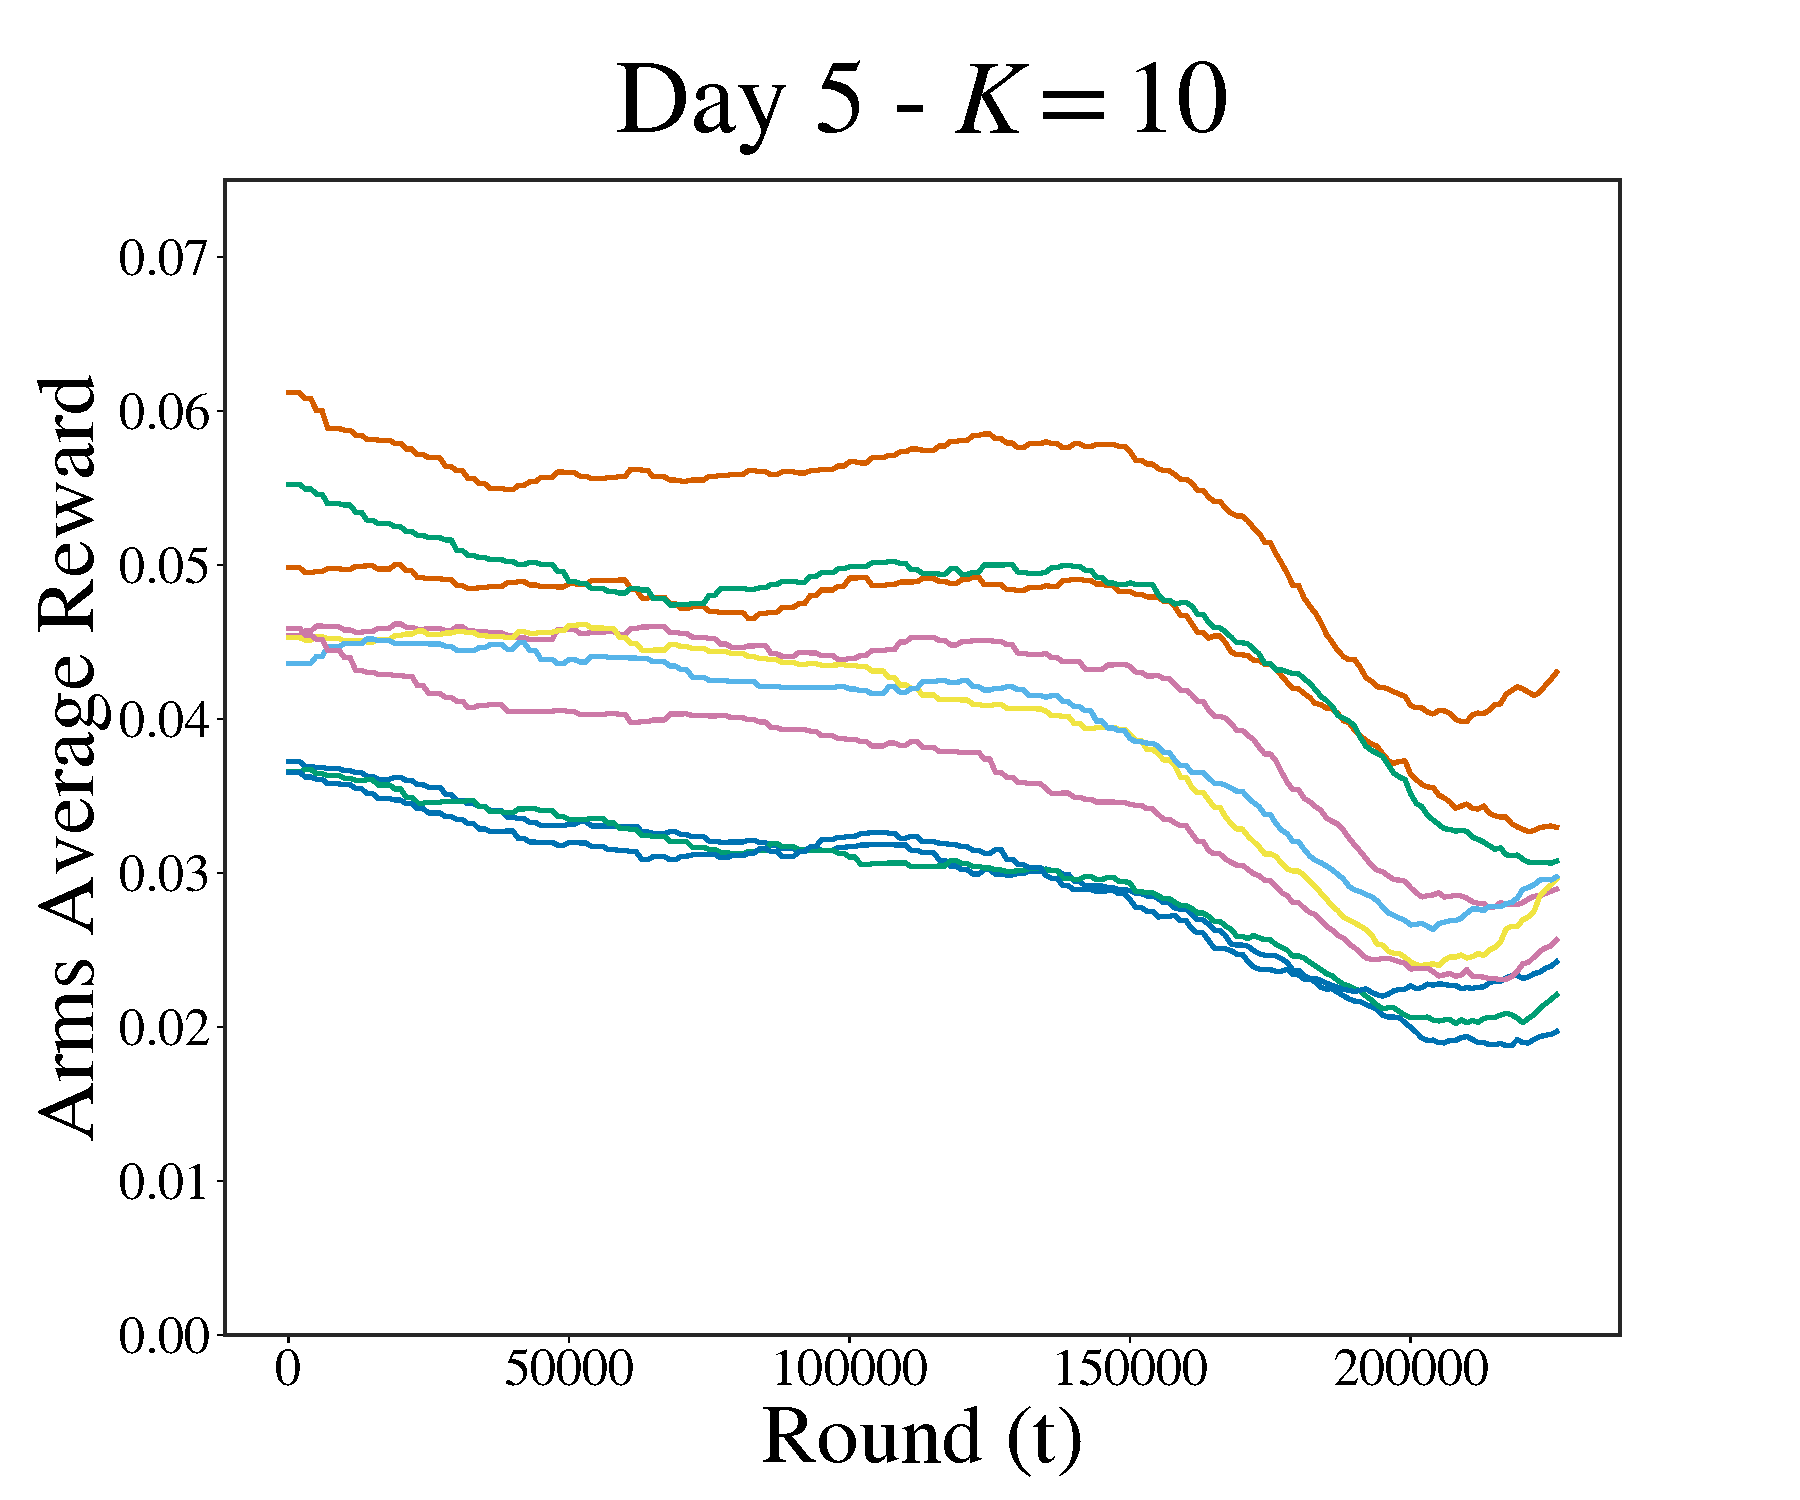
\includegraphics[clip, width= 0.495\textwidth]{4Restless/fig/reward_plot_day5.pdf}
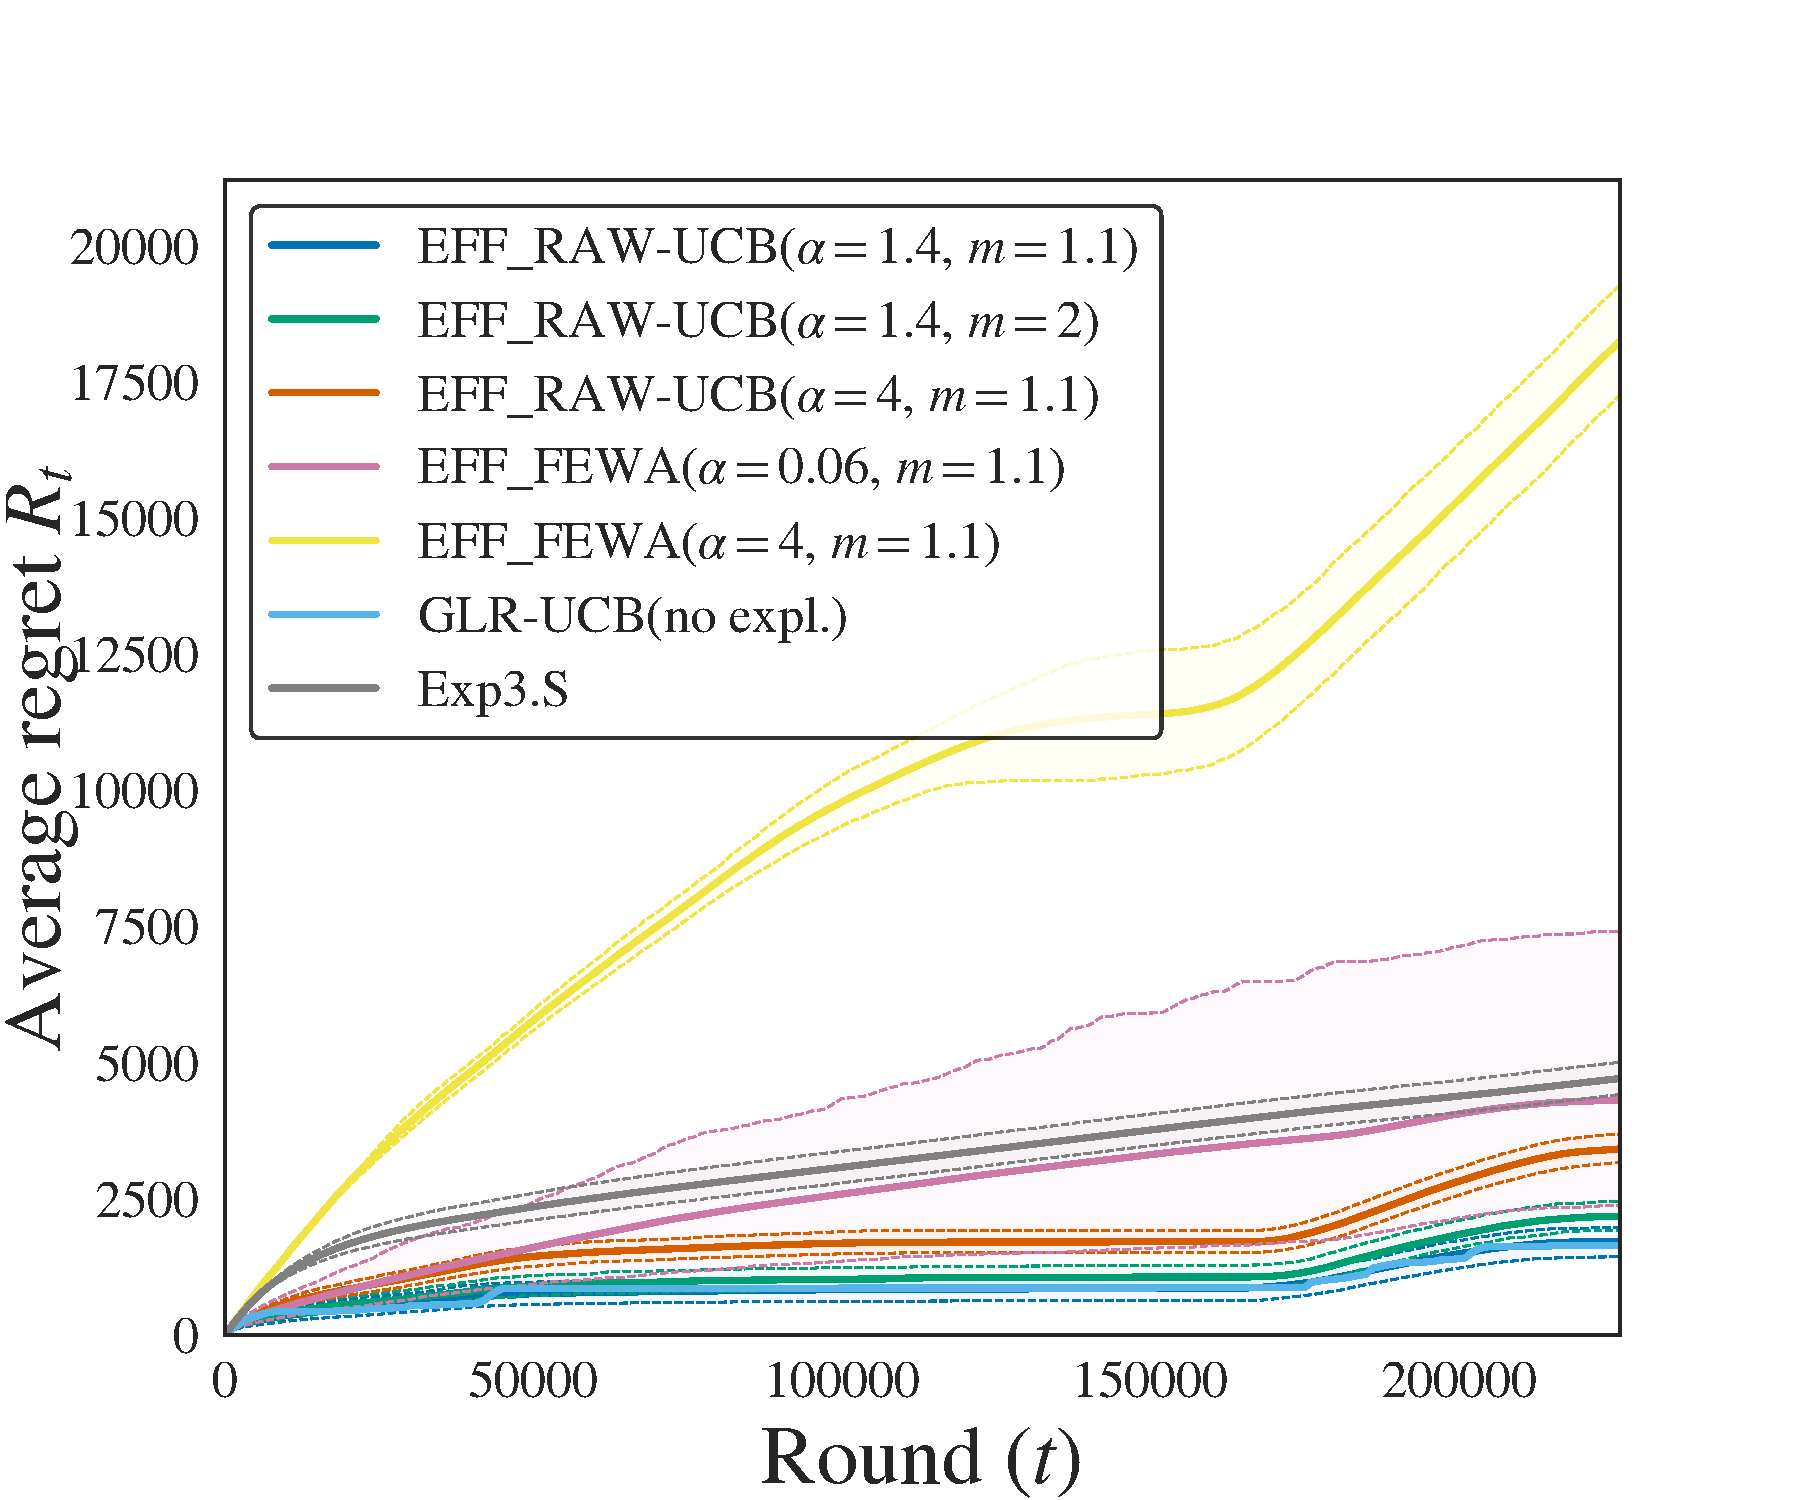
\includegraphics[clip, width= 0.495\textwidth]{4Restless/fig/DAY5.pdf}
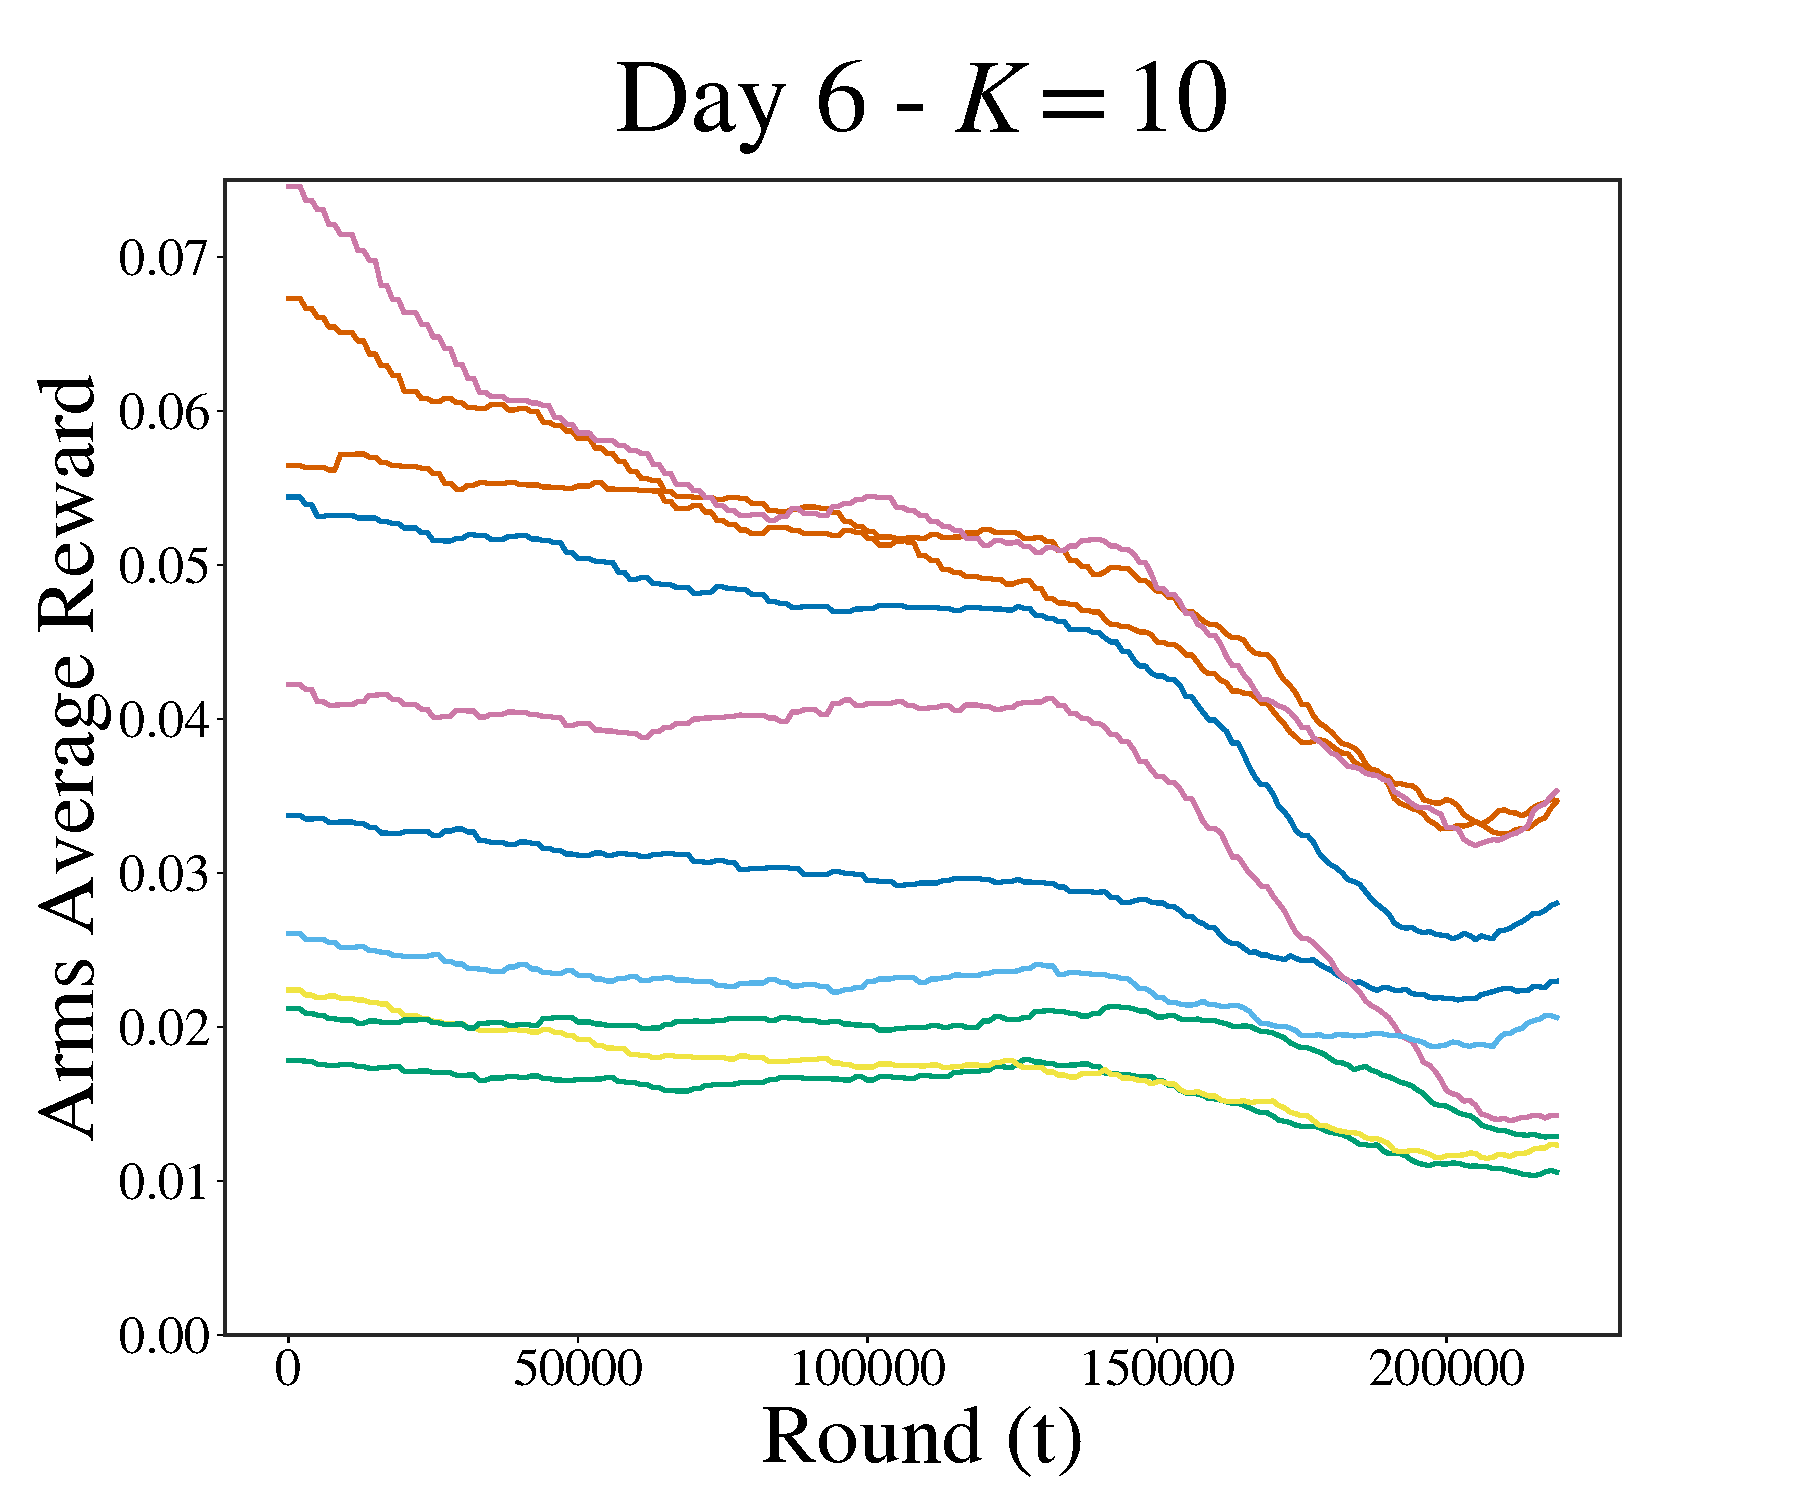
\includegraphics[clip, width= 0.495\textwidth]{4Restless/fig/reward_plot_day6.pdf}
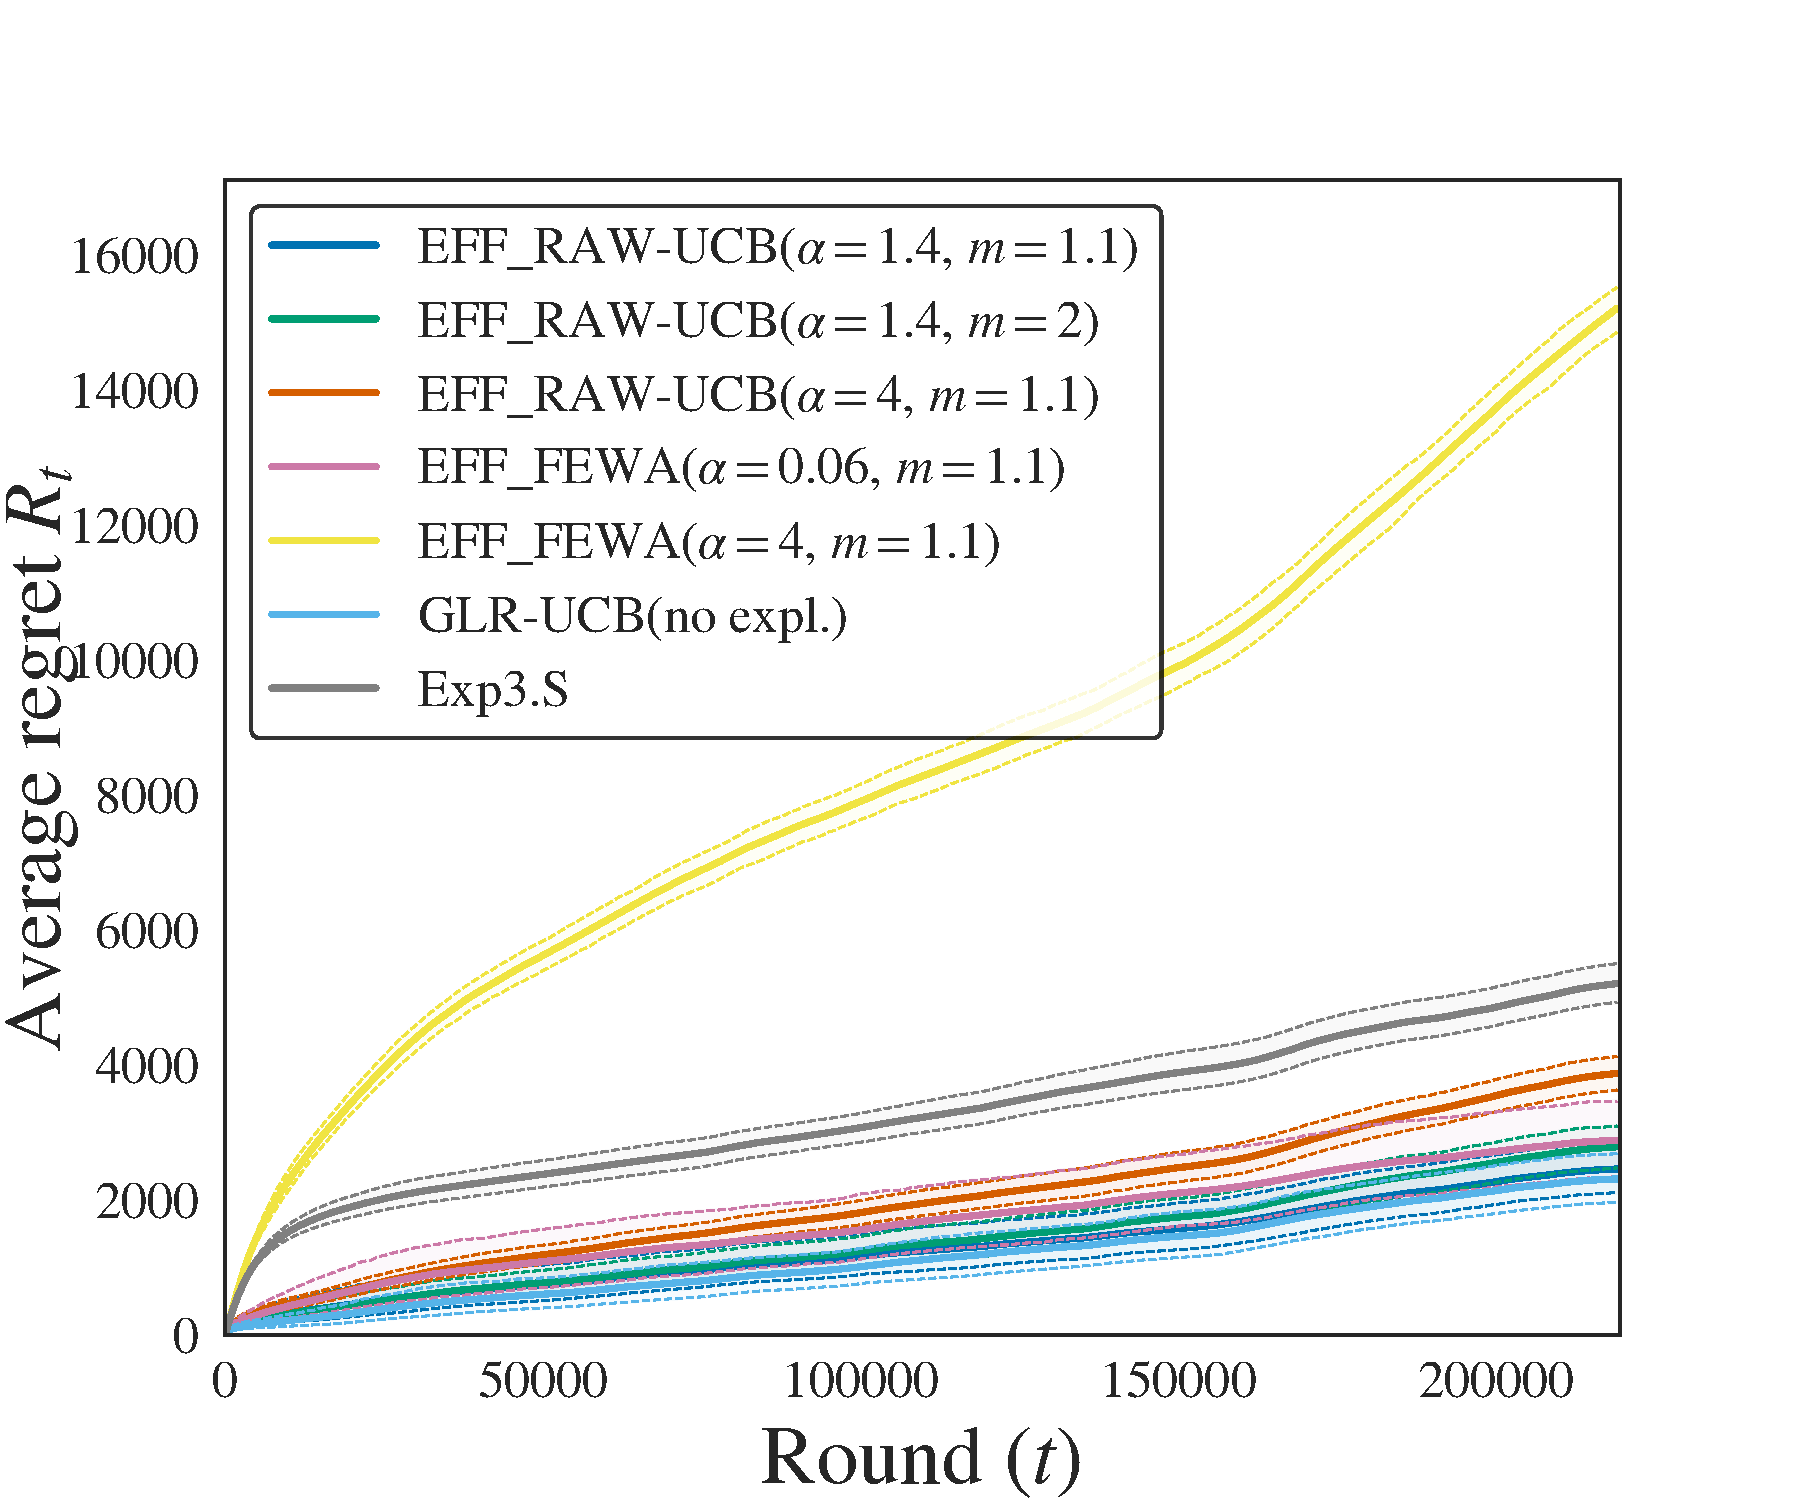
\includegraphics[clip, width= 0.495\textwidth]{4Restless/fig/DAY6.pdf}
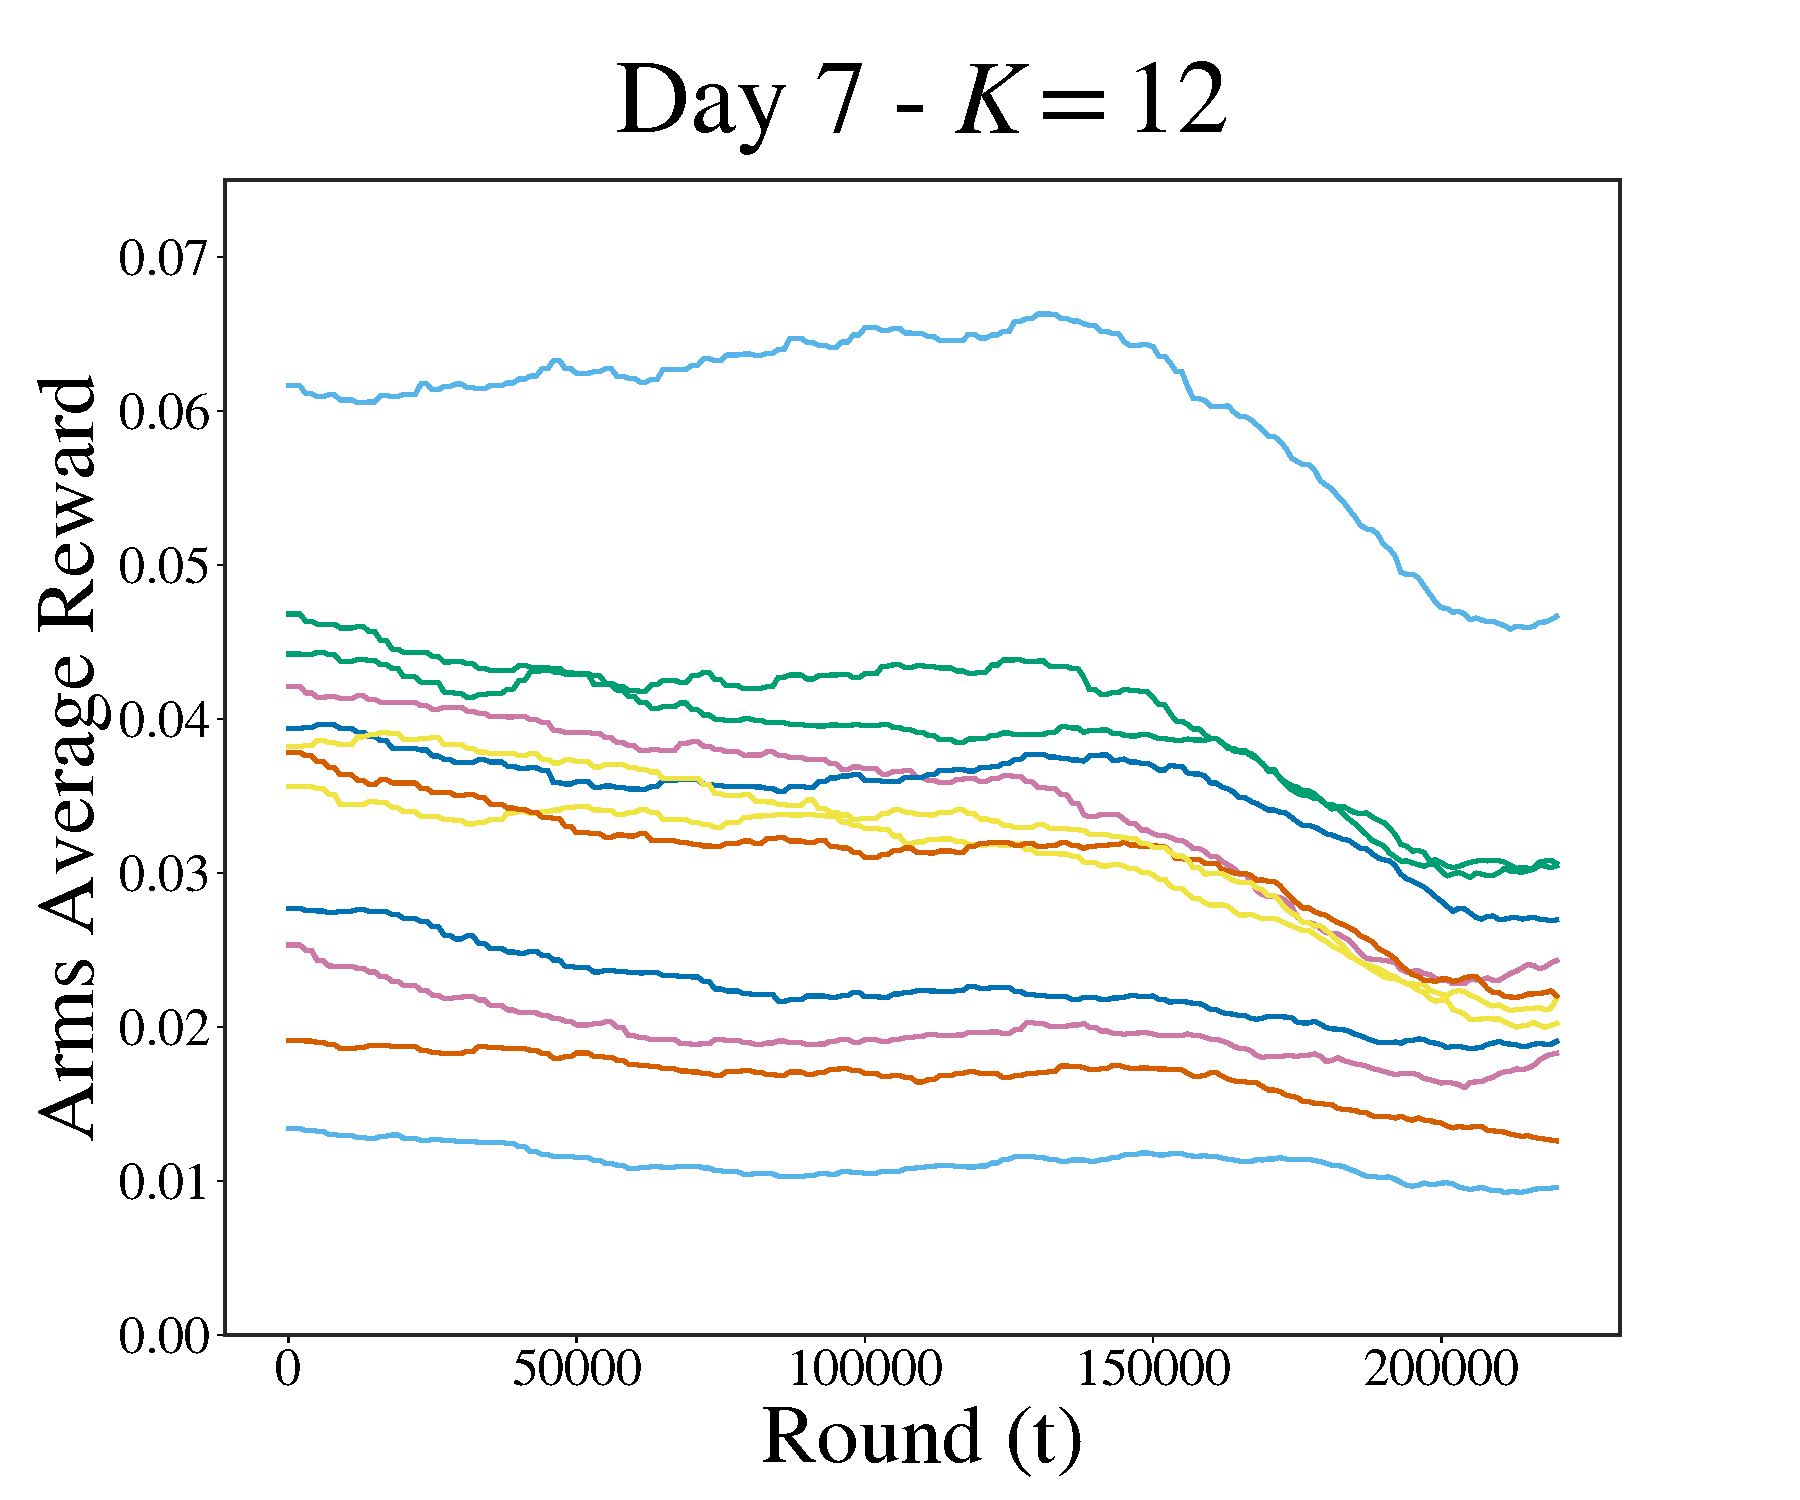
\includegraphics[clip, width= 0.495\textwidth]{4Restless/fig/reward_plot_day7.pdf}
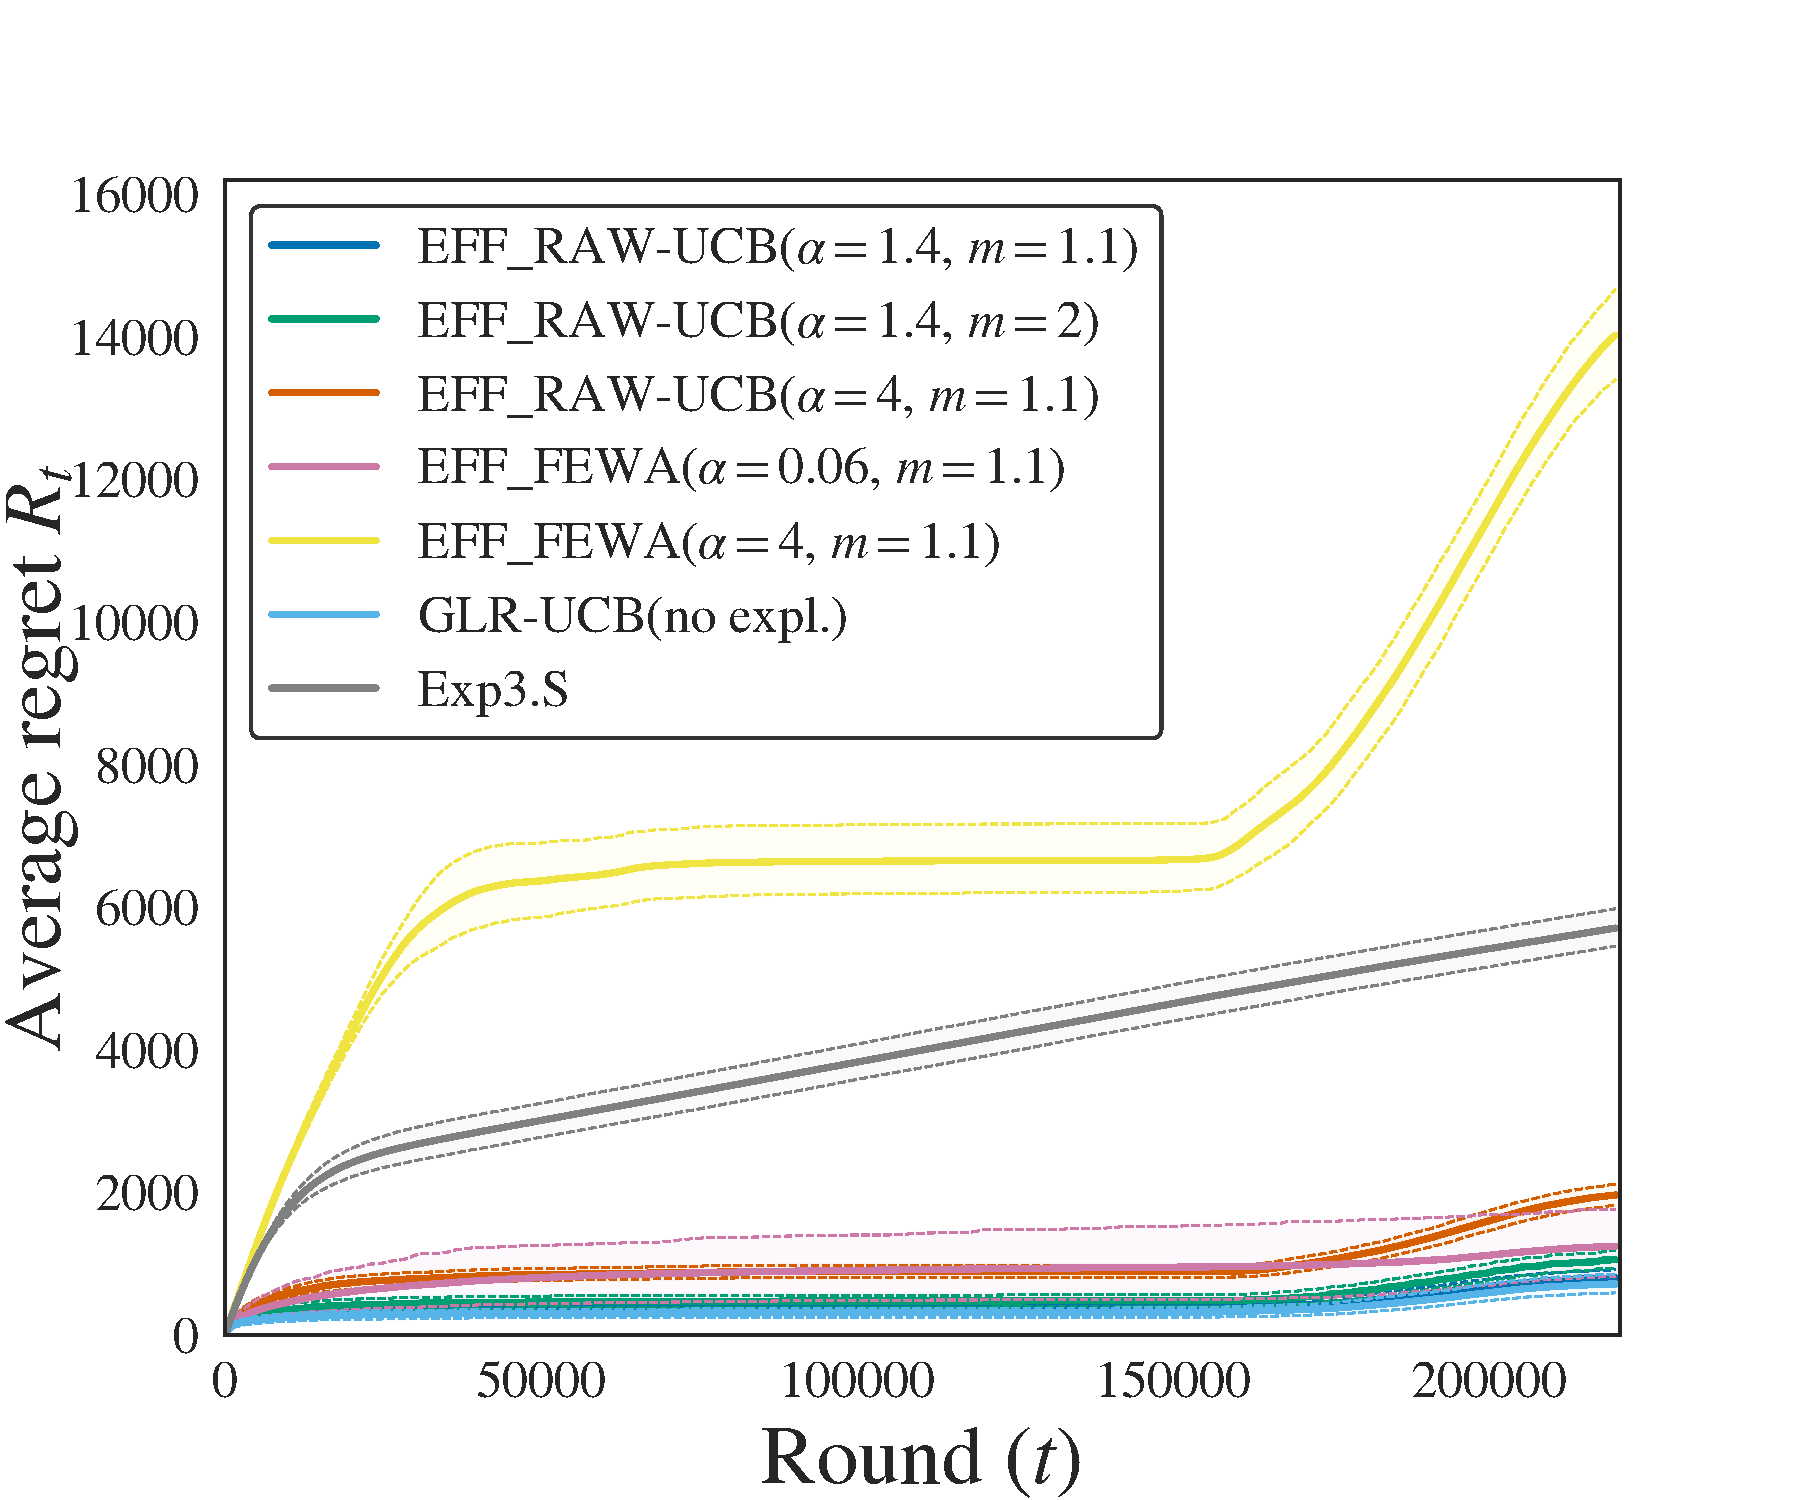
\includegraphics[clip, width= 0.495\textwidth]{4Restless/fig/DAY7.pdf}
\end{figure*}
\begin{figure*}[p!]
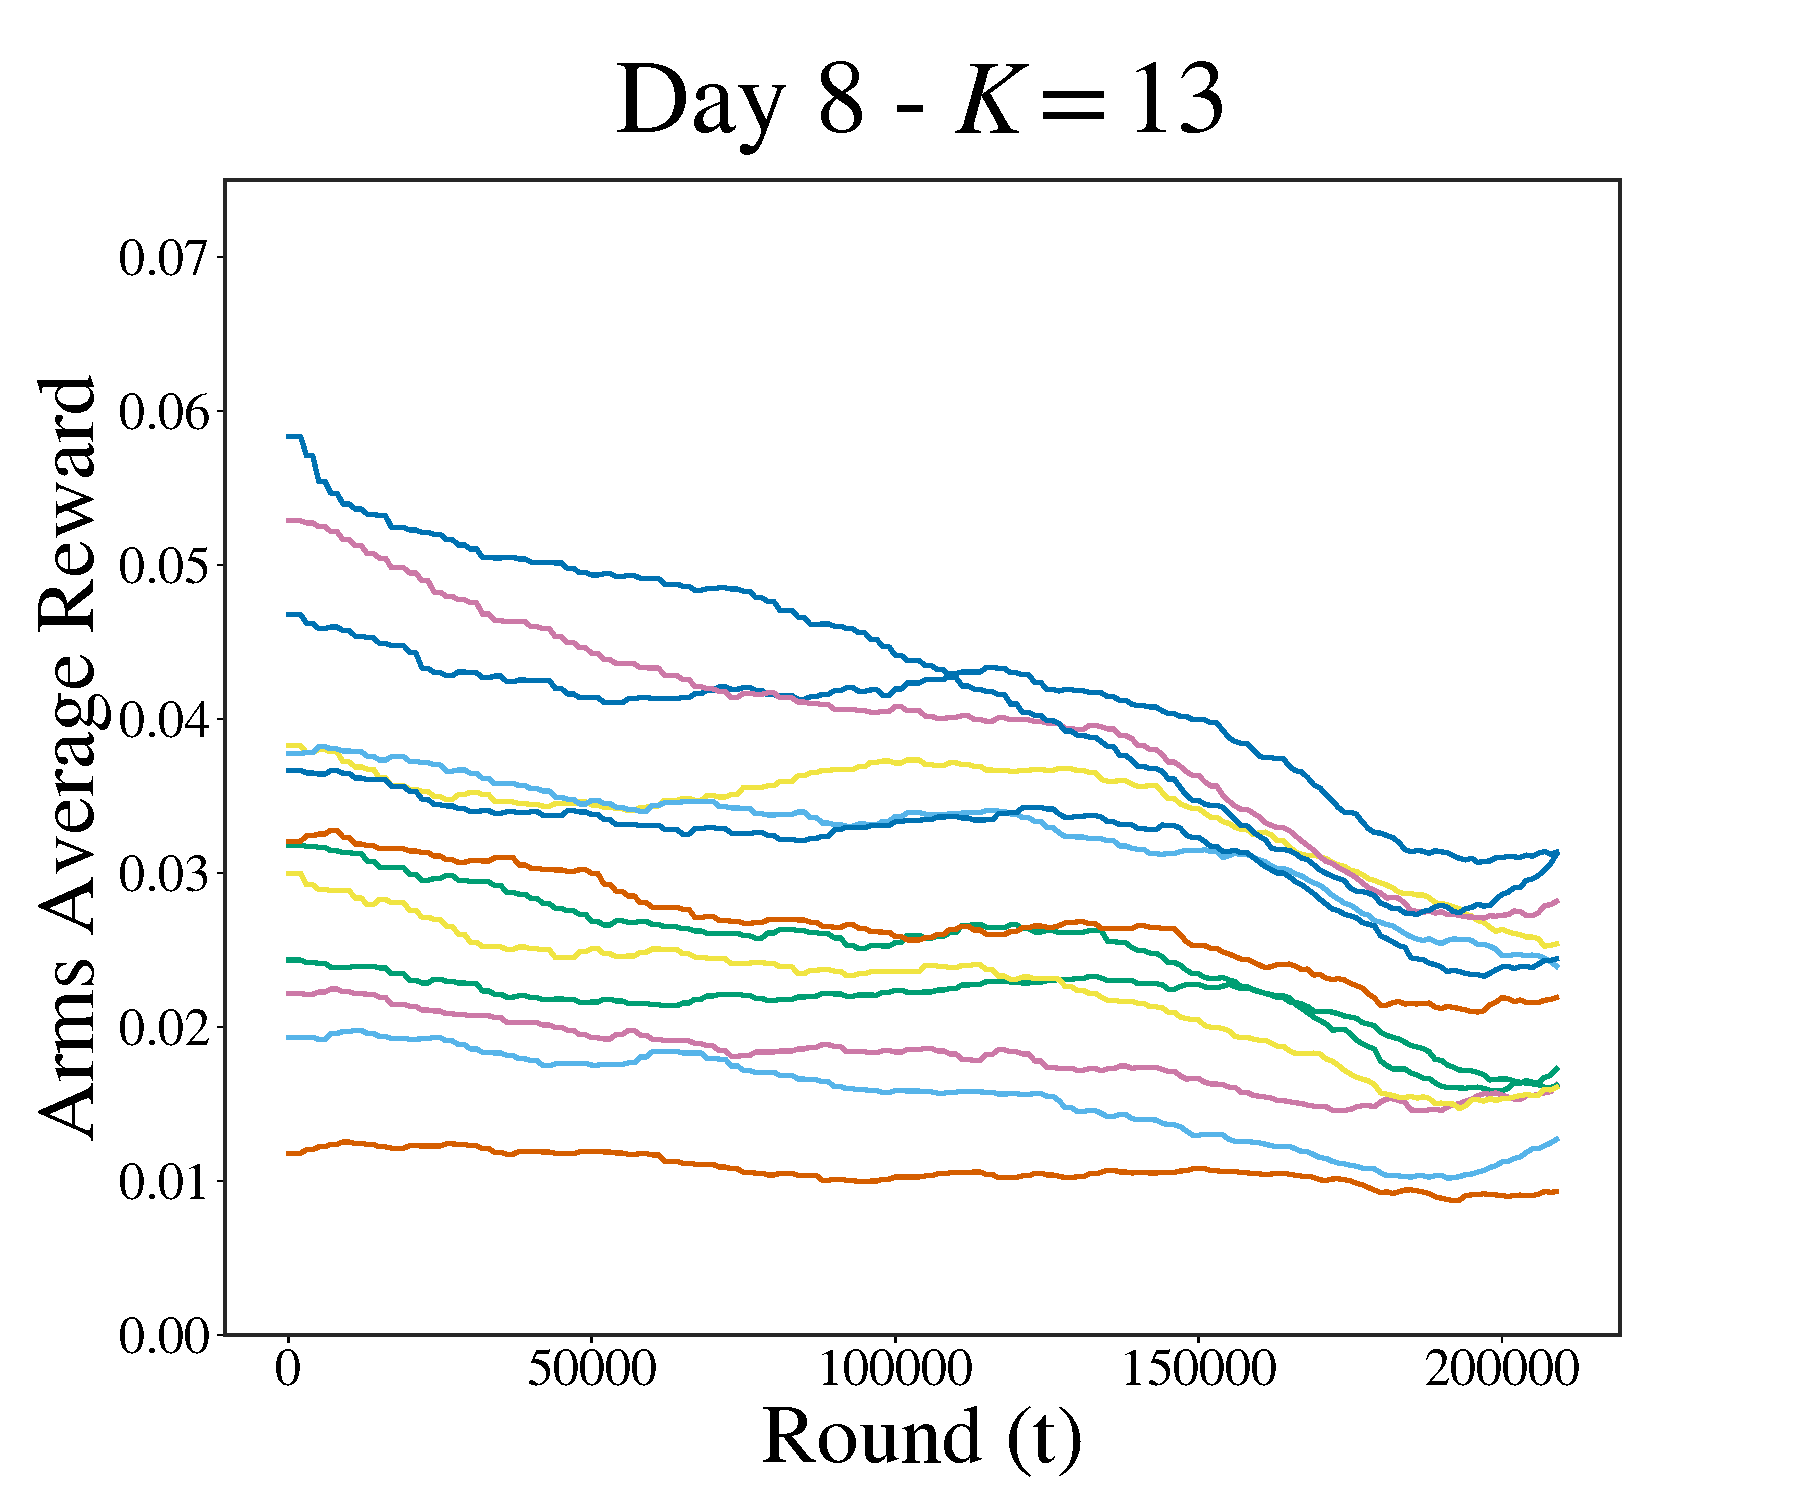
\includegraphics[clip, width= 0.495\textwidth]{4Restless/fig/reward_plot_day8.pdf}
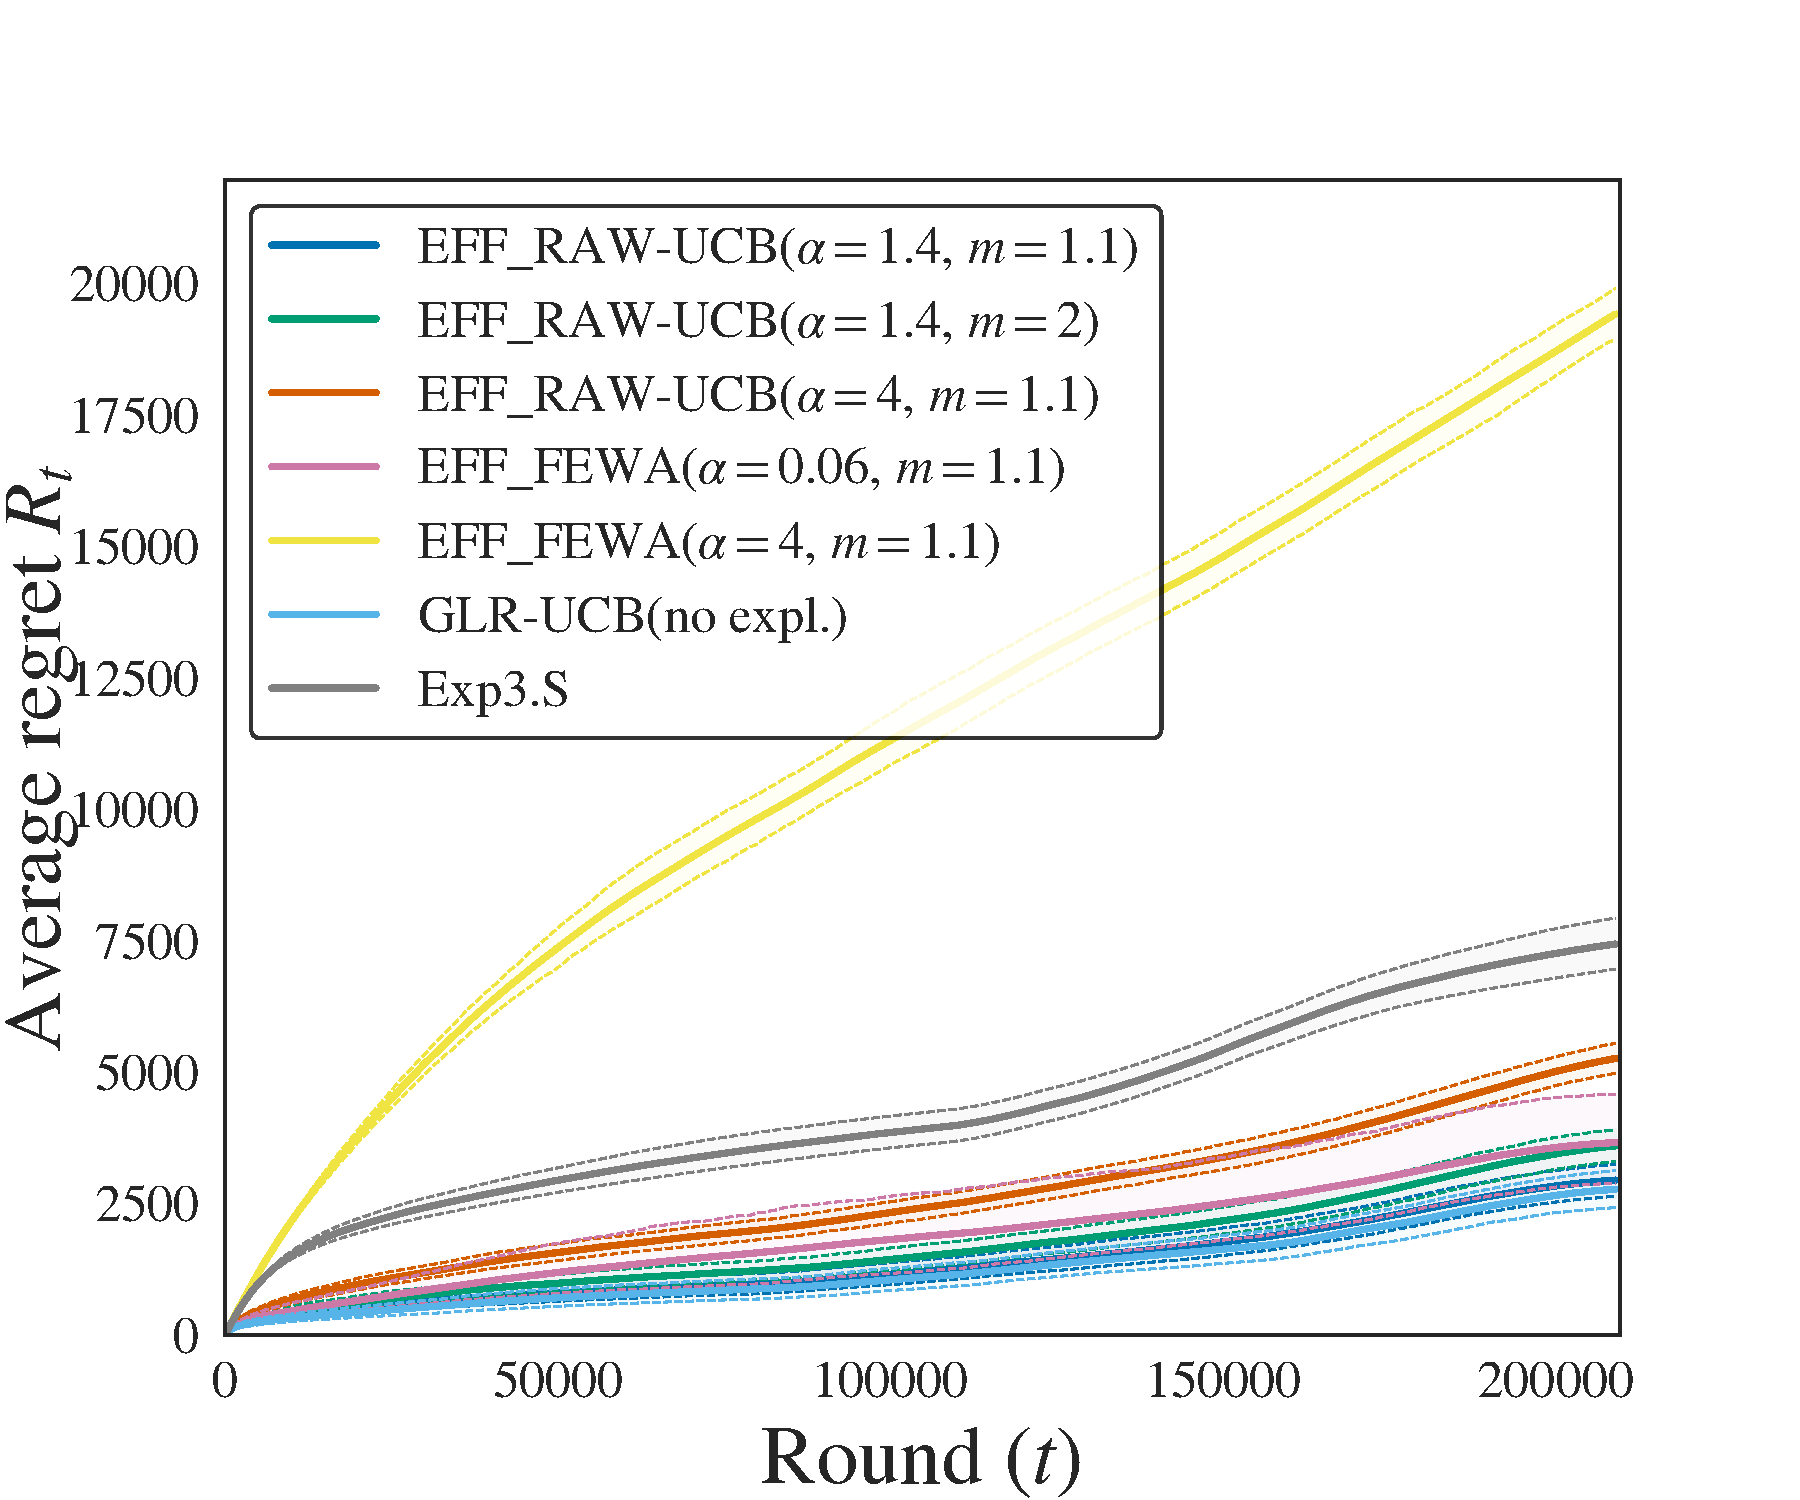
\includegraphics[clip, width= 0.495\textwidth]{4Restless/fig/DAY8.pdf}
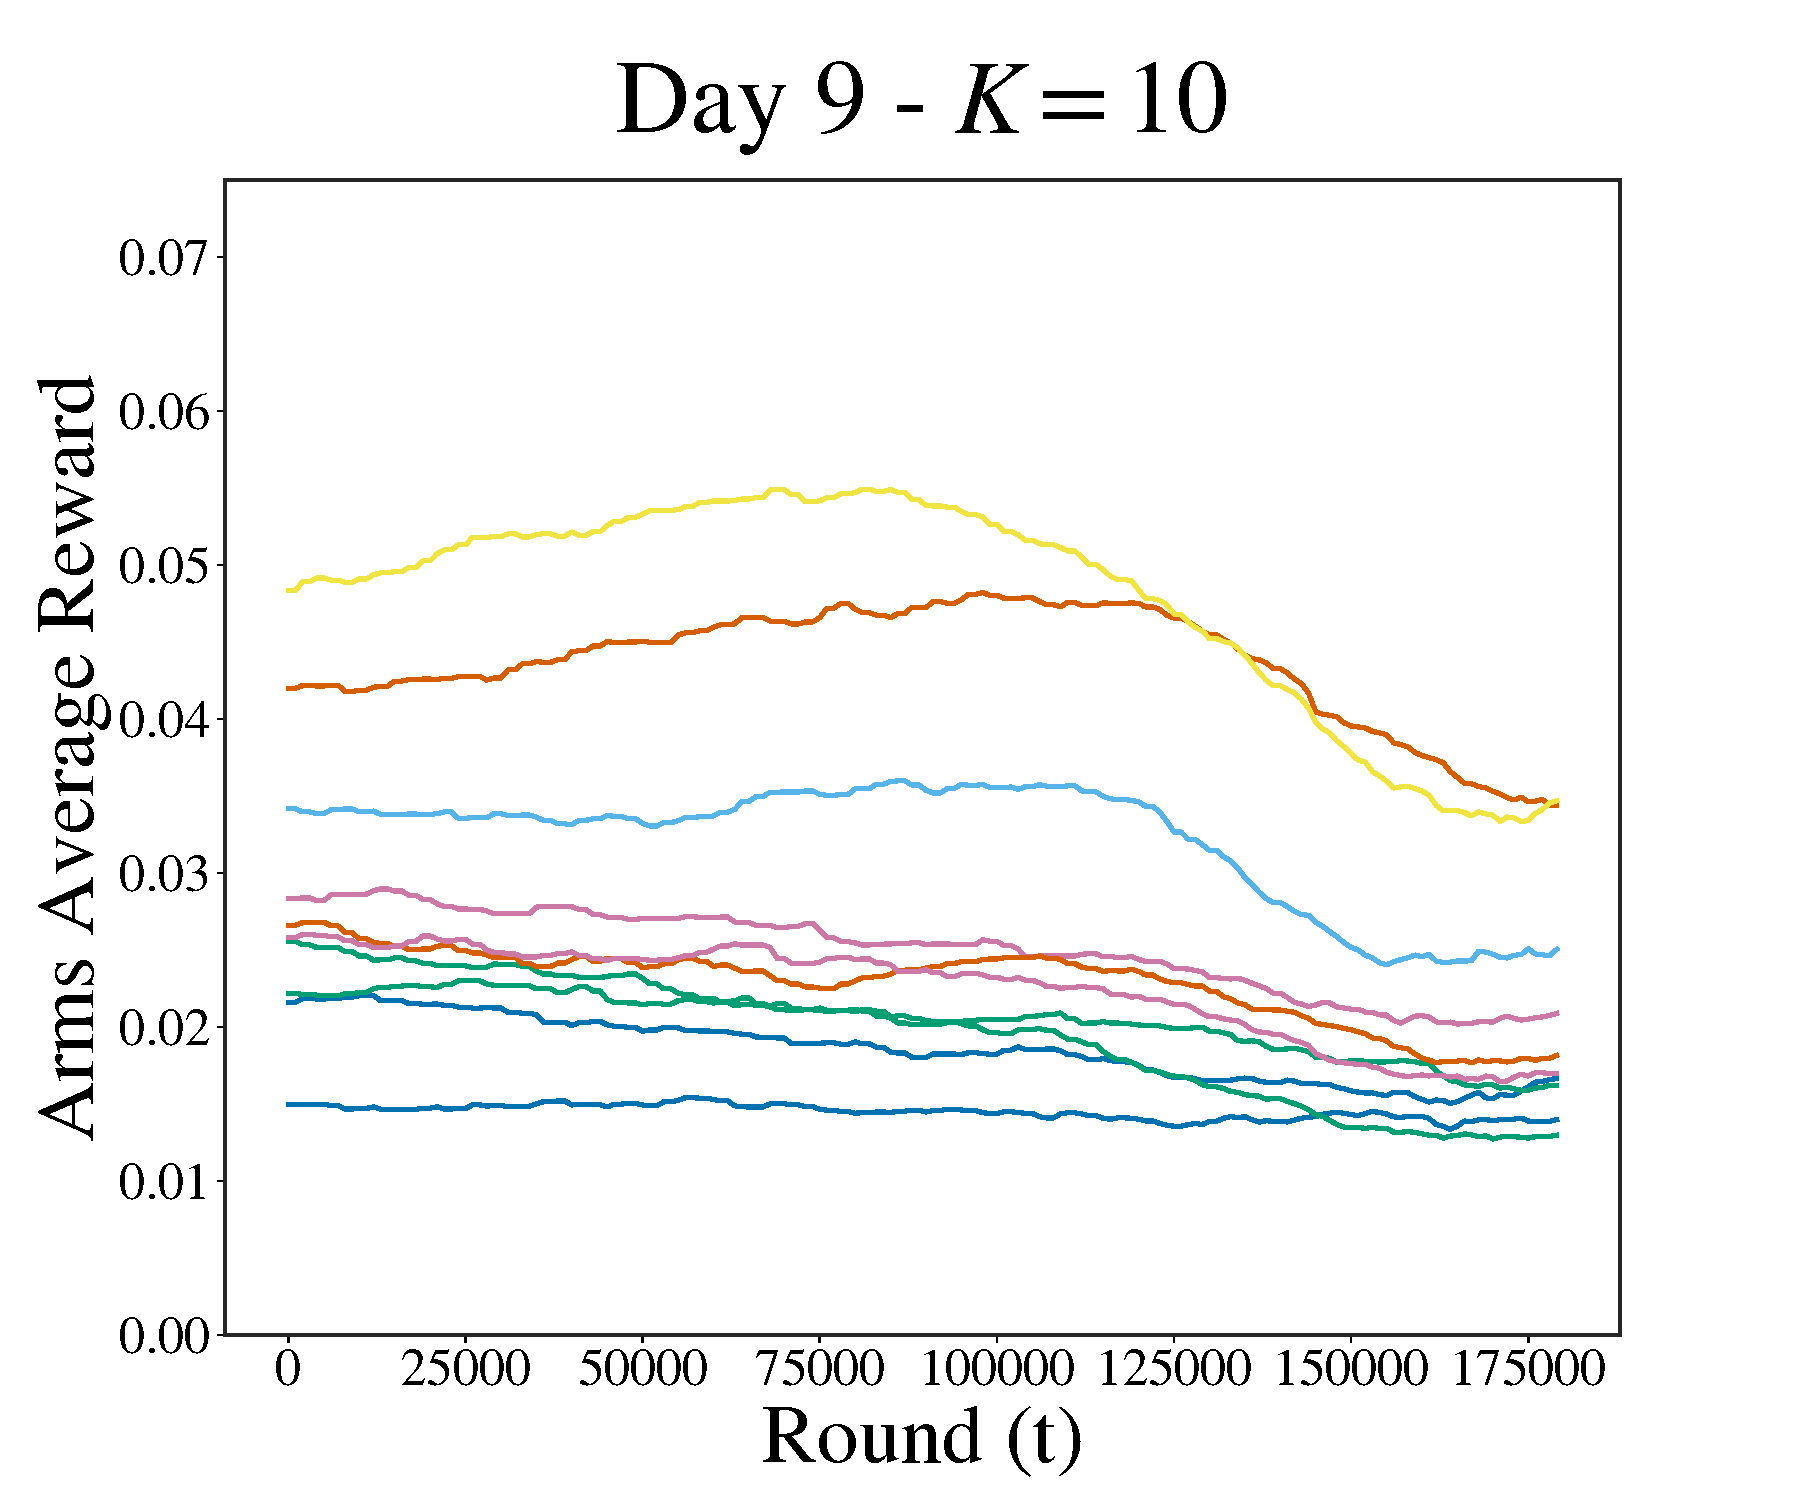
\includegraphics[clip, width= 0.495\textwidth]{4Restless/fig/reward_plot_day9.pdf}
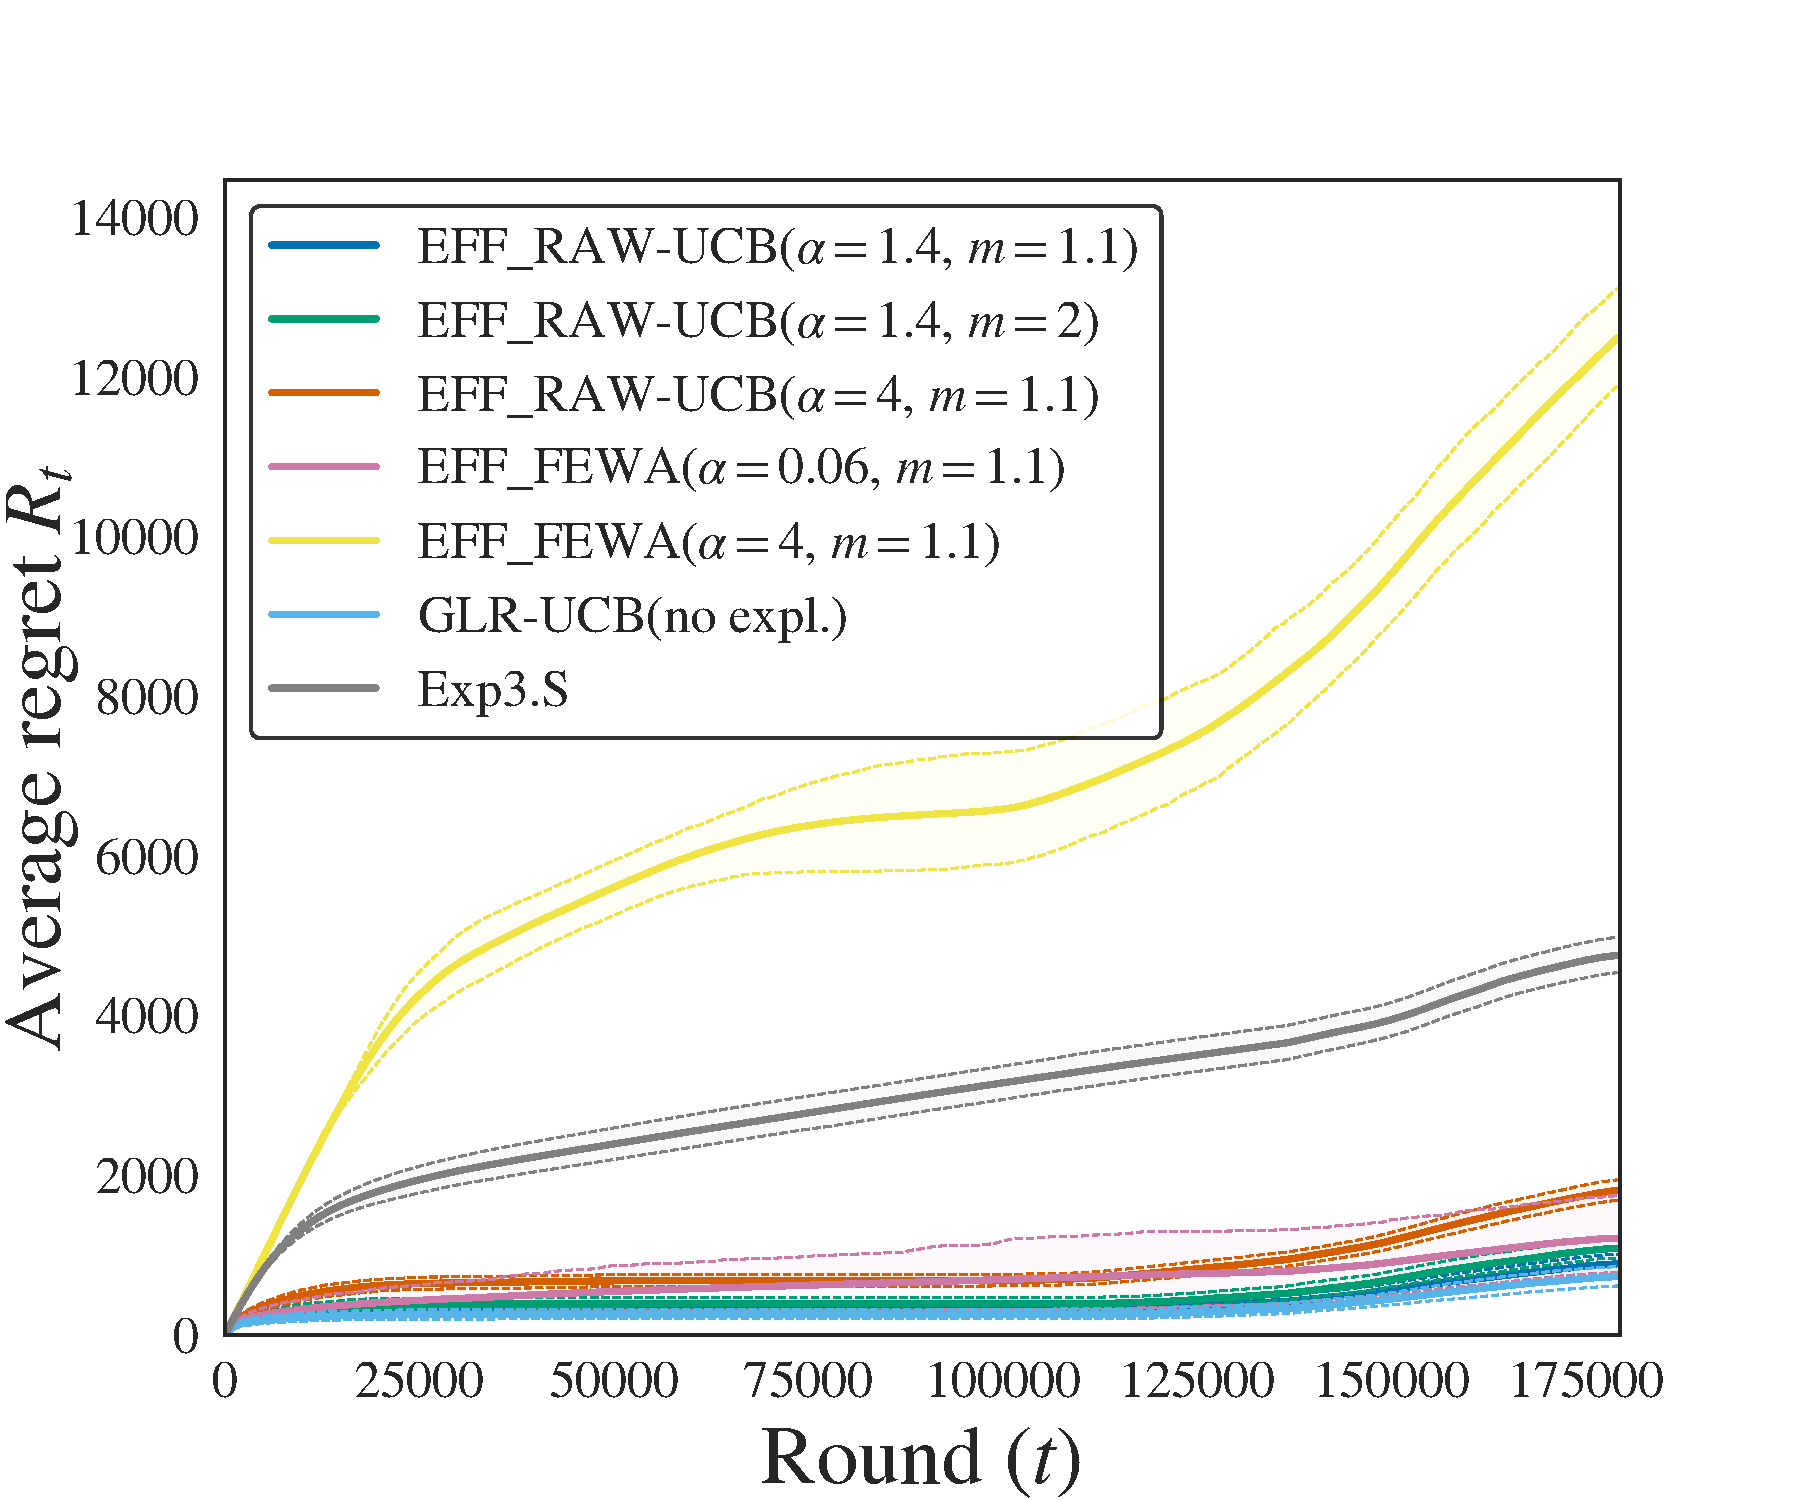
\includegraphics[clip, width= 0.495\textwidth]{4Restless/fig/DAY9.pdf}
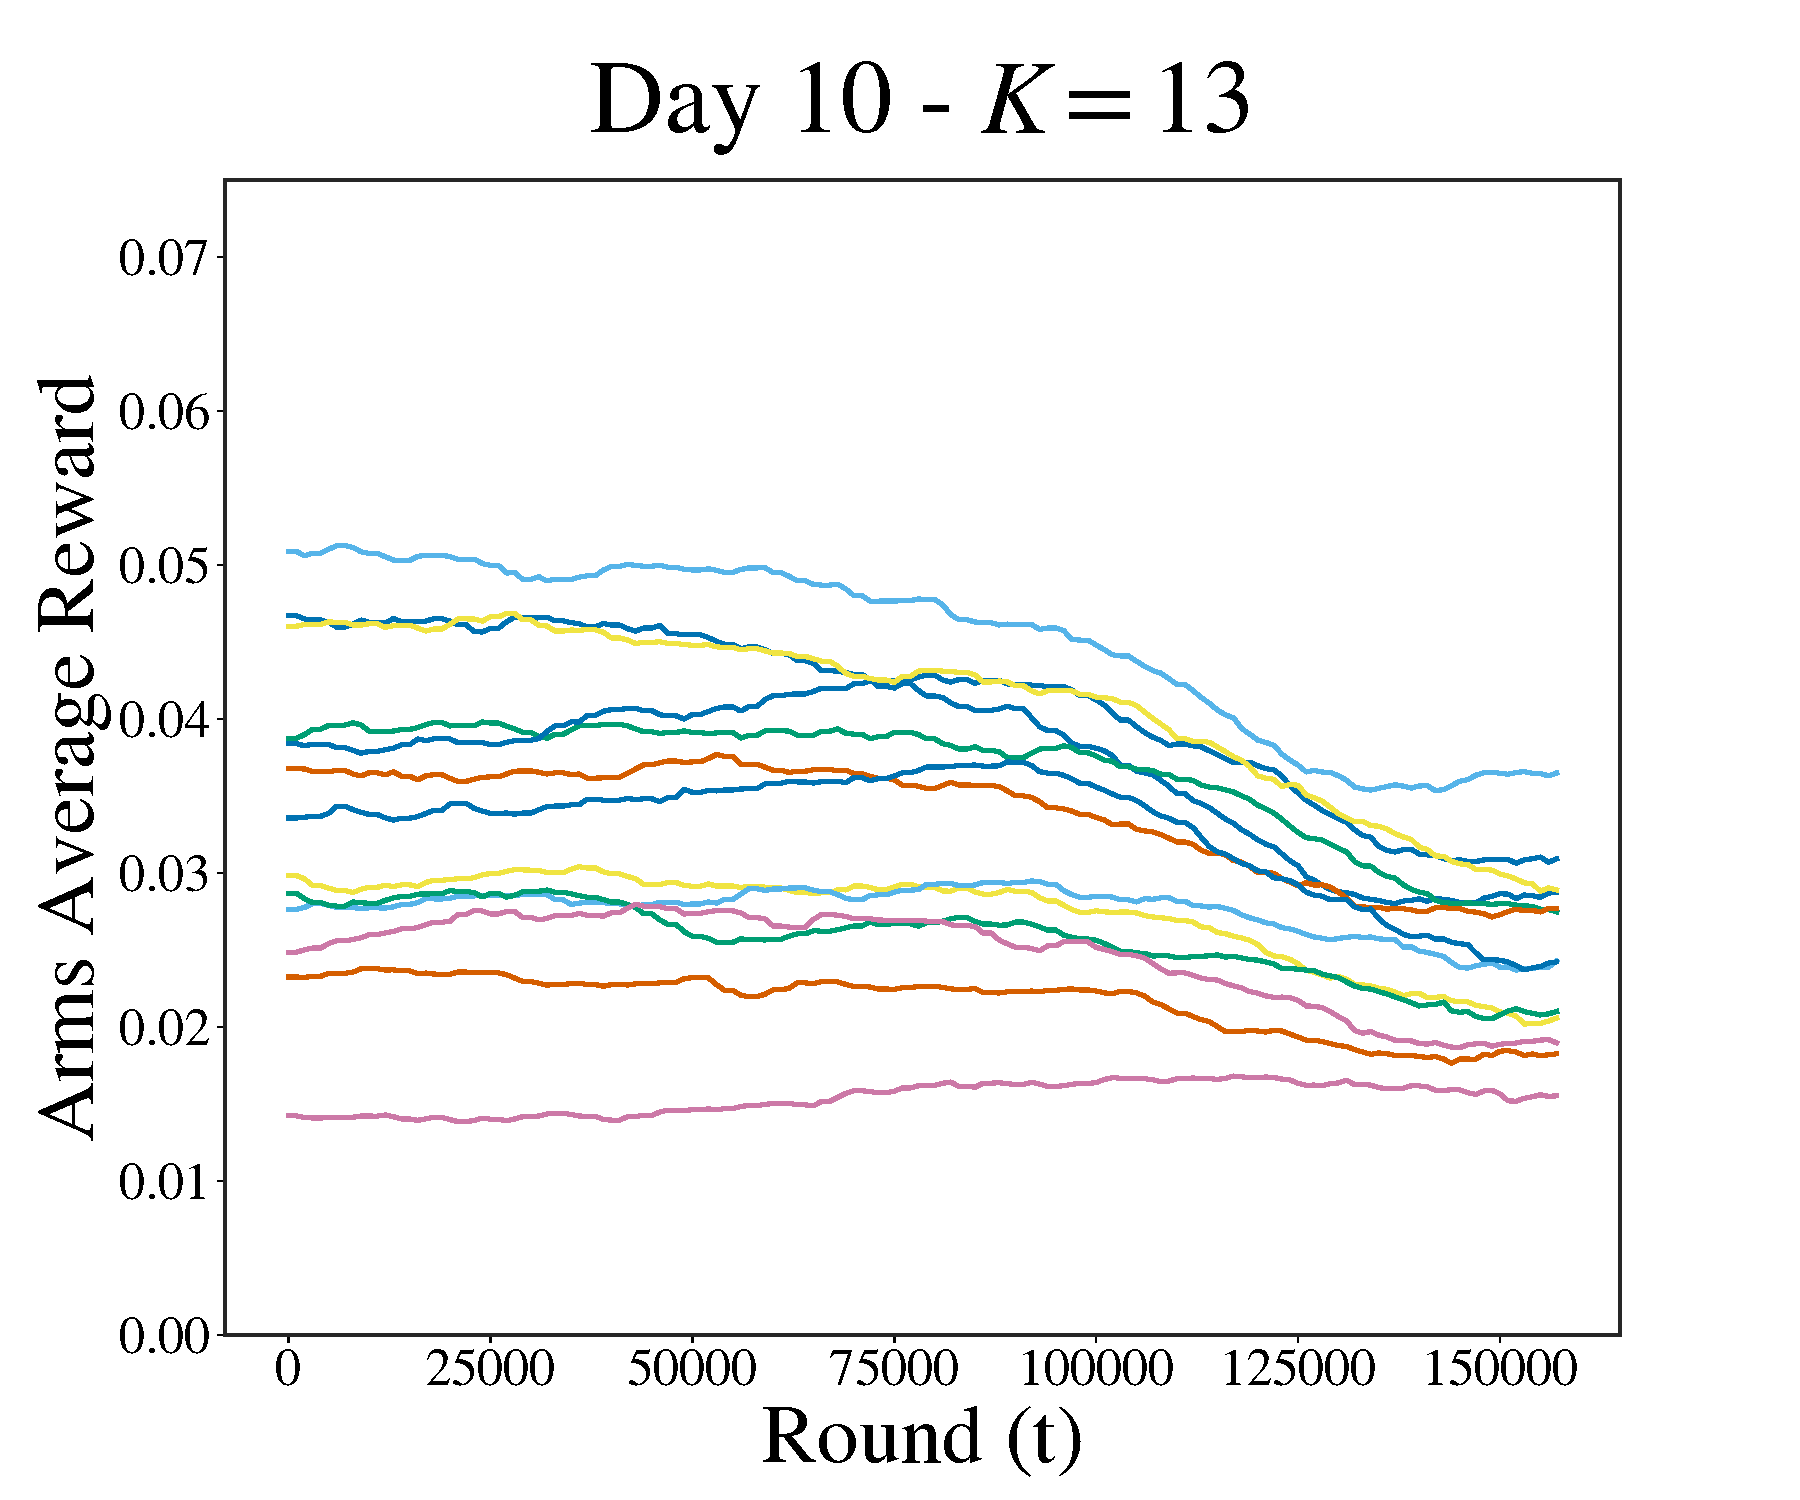
\includegraphics[clip, width= 0.495\textwidth]{4Restless/fig/reward_plot_day10.pdf}
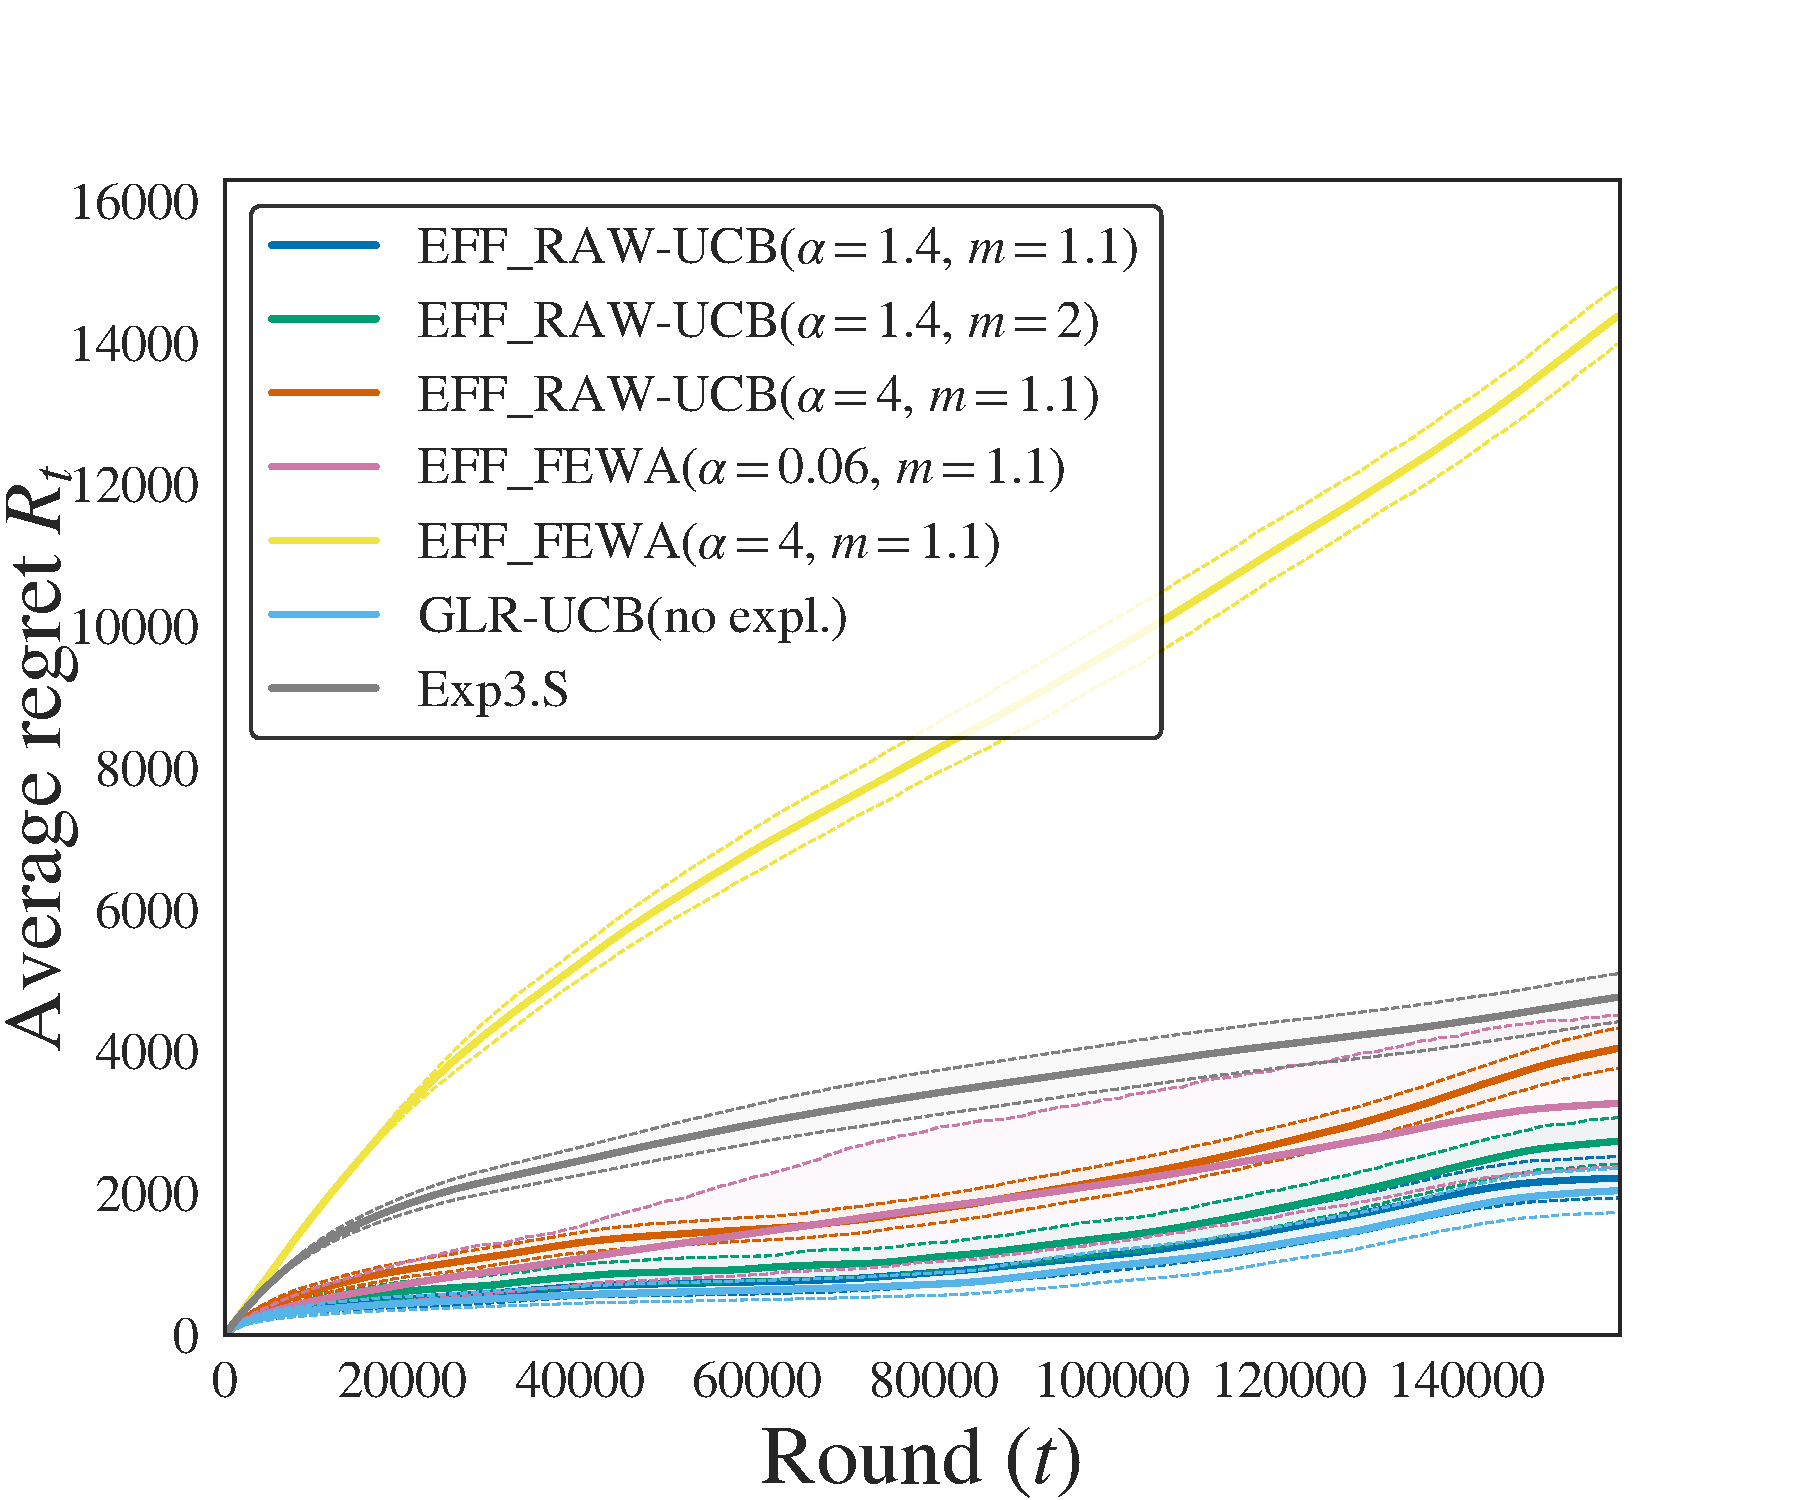
\includegraphics[clip, width= 0.495\textwidth]{4Restless/fig/DAY10.pdf}
\end{figure*}
\begin{table*}[ht!]
\begin{center}
\begin{tabular}{|@{\hskip3pt}c@{\hskip3pt}|@{\hskip5pt}c@{\hskip5pt}|@{\hskip5pt}c@{\hskip5pt}|@{\hskip5pt}c@{\hskip5pt}|@{\hskip5pt}c@{\hskip5pt}|@{\hskip5pt}c@{\hskip5pt}|@{\hskip5pt}c@{\hskip5pt}|@{\hskip5pt}c@{\hskip5pt}|@{\hskip5pt}c@{\hskip5pt}|@{\hskip5pt}c@{\hskip5pt}|}
\hline
\textbf{Day} & \textbf{2} & \textbf{3} & \textbf{4} & \textbf{5} & \textbf{6} & \textbf{7} & \textbf{8} & \textbf{9}              & \textbf{10}               \\ \hline
\!\EFFRAW\! \footnotesize{$\!(\alpha\!=\!1.4, m\!=\!1.1)\!$} \!& 67         & 66         & 90         & 86         & 91         & 74         & 88         & 64 & 48 \\  
\!\EFFRAW\!  {\footnotesize$(\alpha\!=\!1.4, m\!=\!2)$} \!  & 35         & 33         & 43         & 47         & 46         & 41         & 44         & 34   & 45 \\  
\!\EFFRAW \!{\footnotesize $(\alpha\!=\!4, m\!=\!1.1)$}\!   & 65         & 65         & 90         & 88         & 91         & 74         & 89         & 63 & 48  \\ \hline
\EFFFEWA \footnotesize{$(\alpha\!=\!0.06)$}           & 143        & 175        & 223        & 159        & 183        & 115        & 193        & 116        &       165       \\ 
\EFFFEWA \footnotesize{$(\alpha\!=\!4)$}              & 337        & 308        & 391        & 473        & 487        & 380        & 428        & 341     &  388               \\ \hline 
\EXPS   & 56         & 53         & 67         & 77         & 75         & 69         & 71         & 55      &   78 \\ \hline
\GLRUCB  & 560        & 613        & 683        & 2421       & 707        & 1529       & 957        & 971  & 4017\\ \hline
\end{tabular}
  \caption{Average computational time in seconds for each algorithm in each experiment.}
  \label{tab:restless-time}
\end{center}
\end{table*}

\paragraph{{\RAWUCB} vs {\FEWA}.} The two algorithms compute the same statistics and share most of their analysis. Yet, {\RAWUCB} consistently outperforms {\FEWA} as it was the case on the rested benchmark. The difference between the two is even more significant in the restless case. Its theoretical tuning $\alpha = 4$ gets reasonable results, while theoretical {\FEWA} is impractical. Finally, its empirical tuning $\alpha_{\mathrm{R}} =1.4$ is similar to the asymptotic optimal tuning of {\UCB} and shows good performance on both rested and restless problems. By contrast, {\FEWA} with $\alpha_{\mathrm{F}} = 0.06$ shows worse performance with larger deviation on the restless benchmark. 

\paragraph{{\RAWUCB} vs {\EXPS}.} {\EXPS} has good performances on the restless benchmark, on which it has theoretical guarantees. Yet, it is consistently outperformed by {\RAWUCB} when we tune the confidence bounds. It is particularly true in easy instances, e.g. on day 7. Indeed, in these cases, we expect a logarithmic regret rate for {\RAWUCB}.

\paragraph{{\RAWUCB} vs {\GLRUCB} (no active exploration).}  On the restless benchmark, {\GLRUCB} shows similar results than {\RAWUCB}. Yet, we highlight that 1) {\GLRUCB} needs the knowledge of the horizon to tune its change-detector; 2) we use an efficient version of {\RAWUCB} which runs $\sim 10$ times faster than {\GLRUCB}. In fact, the two algorithms are similar: they are UCB index policies, they recover logarithmic rate on easy restless rotting bandits problems and hence they would both suffer near-linear worst-case regret rate in the general restless setting (when active exploration is turned off for {\GLRUCB}). The main difference is that {\RAWUCB} scans its history to select its rotting UCB's window, while {\GLRUCB} scans its history to detect significant changes and restart. 

